%
% PROJECT: <ETD> Electronic Thesis and Dissertation Initiative
%   TITLE: LaTeX report template for ETDs in LaTeX
%  AUTHOR: Neill Kipp, nkipp@vt.edu
%     URL: http://etd.vt.edu/latex/
% SAVE AS: etd.tex
% REVISED: September 6, 1997 [GMc 8/30/10]
% 

% Instructions: Remove the data from this document and replace it with your own,
% keeping the style and formatting information intact.  More instructions
% appear on the Web site listed above.

\documentclass[12pt]{report}

\usepackage{fullpage}
\usepackage{natbib}
%\usepackage{breakurl}
\usepackage{algorithmic}
\usepackage{alltt}
\usepackage[ruled]{algorithm2e}
\usepackage[cmex10]{amsmath}
\usepackage{url} 
\usepackage{graphicx}
\usepackage{listings}
\usepackage{wrapfig}
\usepackage{multirow}
%\usepackage[plainpages=false, colorlinks=true, urlcolor={cyan}, citecolor={red}, linkcolor={green}]{hyperref}
\usepackage[plainpages=false]{hyperref}
\usepackage{array}
\usepackage{balance}
\usepackage{subfigure}
\usepackage{amssymb}
\usepackage{float}
%\usepackage{caption}
\usepackage{placeins}
\usepackage{harmony}
\usepackage{pdfpages}

% % % % % % % % % % % % % % % % % % % % % % % % % % % % % % % % 
\lstset{frame=none, xleftmargin=15pt, stepnumber=1, numbers=left, numbersep=5pt,
numberstyle=\tiny, belowcaptionskip=\bigskipamount,
captionpos=b, escapeinside={*'}{'*}, language=java, tabsize=2, emphstyle={\bf},
commentstyle=\it, stringstyle=\mdseries\ttfamily, showspaces=false,
keywordstyle=\bfseries, morekeywords={in,do,print,Metadata,Where}, columns=flexible,
basicstyle=\footnotesize\ttfamily, showstringspaces=false, morecomment=[l], mathescape=true}



% \newcommand{\solution}{\bigskip\hrule\bigskip}
% \newcommand{\problembreak}{\bigskip\hrule\bigskip}

% \renewcommand{\theenumi}{\bf\Alph{enumi}}

% \newlength{\spread}
% \setlength{\spread}{1.0in}

% \def\bibfont{\footnotesize}

% correct bad hyphenation here
%\hyphenation{op-tical net-works semi-conduc-tor}


%%%%%%%%%%%%%%%%%%%%%%% END of LaTeX definitions %%%%%%%%%%%%%%%%%%%%%%%%%%%%

\setlength{\textwidth}{6.5in}
\setlength{\textheight}{8.5in}
\setlength{\evensidemargin}{0in}
\setlength{\oddsidemargin}{0in}
\setlength{\topmargin}{0in}

\setlength{\parindent}{0pt}
\setlength{\parskip}{0.1in}
\setlength{\headsep}{0.3in}

% Uncomment for double-spaced document.
% \renewcommand{\baselinestretch}{2}

% \usepackage{epsf}

\begin{document}

\thispagestyle{empty}
\pagenumbering{roman}
\begin{center}

% TITLE
{\Large 
Musiplectics: Computational Assessment of the Complexity of Music Scores
}

\vfill

Ethan G. Holder

\vfill

Dissertation submitted to the Faculty of the \\
Virginia Polytechnic Institute and State University \\
in partial fulfillment of the requirements for the degree of

\vfill

Master of Science \\
in \\
Computer Science

\vfill

Eli Tilevich, Chair \\
Amy Gillick \\
R. Ben Knapp

\vfill

April 23, 2015 \\
Blacksburg, Virginia

\vfill

Keywords: Music Scores; Music Complexity Assessment; Novel Computing Domains; MusicXML
\\
Copyright 2015, Ethan G. Holder

\end{center}

\pagebreak

\thispagestyle{empty}
\begin{center}

{\large Musiplectics: Computational Assessment of the Complexity of Music Scores}

\vfill

Ethan G. Holder

\vfill

(ABSTRACT)

\vfill

\end{center}

In the Western classical tradition, musicians play music from notated sheet music, called a score. When playing music from a score, a musician translates its visual symbols into sequences of instrument-specific physical motions. Hence, a music score's overall complexity represents a sum of the cognitive and mechanical acuity required for its performance.
For a given instrument, different notes, intervals, articulations, dynamics, key signatures, and tempo represent dissimilar levels of difficulty, which vary depending on the performer's proficiency. Individual musicians embrace this tenet, but may disagree about the degrees of difficulty.

This thesis introduces \emph{musiplectics}\footnote{musiplectics = music + plectics, Greek for the study of complexity}, a systematic and objective approach to computational assessment of the complexity of a music score for any instrument. Musiplectics defines computing paradigms for automatically and accurately calculating the complexity of playing a music score on a given instrument. The core concept codifies a two-phase process. First, music experts rank the relative difficulty of individual musical components (e.g., notes, intervals, dynamics, etc.) for different playing proficiencies and instruments. Second, a computing engine automatically applies this ranking to music scores and calculates their respective complexity. As a proof of concept of musiplectics, we present an automated, Web-based application called Musical Complexity Scoring (MCS) for music educators and performers. Musiplectics can engender the creation of practical computing tools for objective and expeditious assessment of a music score's suitability for the abilities of intended performers.

This thesis is based on research submitted for publication at ONWARD'15.

\vfill

% GRANT INFORMATION

That this work received support from a Virginia Tech ICAT SEED grant.

\pagebreak

% Dedication and Acknowledgments are both optional

\chapter*{Dedication}

\thispagestyle{empty}

\begin{center}

\vfill

%This thesis is dedicated to the memories of Robert Brooks Nance, Katherine Gayle Nance, and Durward Alexander Holder. You are deeply loved and sorely missed.  

\textit{To the memory of Coppertone Holder, the standard by which all other pets shall be measured.}

\vfill

\end{center}

\pagebreak

\chapter*{Acknowledgments}

\thispagestyle{empty}

I have not experienced anything in this world quite like the publication of my master's thesis. It has taken only my last two years of graduate school to accomplish, but it has brought me (kicking and screaming at times) further along in those two years than I could have possibly imagined. This process took its toll many times not only on myself, but on all of those close to me. Thus, I'd like to take a moment to graciously acknowledge and thank all of those that had a hand in both shaping my research and keeping my sanity.

I must first thank my parents, Mark and Laurel Holder, without whom I would not even be here. From a very young age, they instilled a love of learning in me and constantly encouraged me, even when I stumbled along my way. You are always a guiding light and a safe harbor in storms. I could write a thesis on this topic alone, but I'll suffice it to say I owe it all to you, and I can never thank you both enough.

My fianc\'ee, my silly, my partner in crime, my goofball, my Baehr, my BMVHB, my coffee-holic, my chocolate monster, my running buddy, my unsung hero... You have all these names to me, but more than each, you are the love of my life Bryanna Baehr. You inspire me in new ways every day and make all of this worth while. I'm so thankful for all the love you give, especially on my worst days. And don't worry, my vows can't possibly be as long as this thesis.

To Logan Patterson, we've been great friends since Kindergarten, when life was so much simpler, all the way up to and beyond our college time. We even managed to live together in a dorm and an apartment for 3 years with two other hooligans. Whether it was bouncing research ideas off of each other and calling out some that weren't up to par or just planning our next hair brained scheme and gaming on xbox, we were together through it all. Although our motives were often simply so we could play more video games later, you've kept me sane and challenged me to perform at my very best, and for that I am always grateful.

To Chris Schmucker, with a name like Schmucker's, it's gotta be good. You've always been there for me when I just needed to vent and escape for a little while. We've also gotten into a fair amount of trouble all around the country from band trips in high school to concerts for other artists. You've even saved my life on at least one occasion. I owe you so much and more. Thank you always and stir the coffee good sir.

One person above all others has been instrumental along my research career. Dr. Eli Tilevich, you've been my advisor and even more to me since my time beginning research as a lowly undergrad when I just wanted a fun project to get some experience. You have guided me through this crazy process and taught me uncountable lessons along the way. I can't say that all of these lessons adhered to conventional wisdom, such as how to determine the true prestige of attending certain conferences based on weather patterns or how to play a great April fools joke on the faculty, but they were nonetheless entertaining and effective. Sometimes lessons could be more eye opening as well. I still remember how much I believed myself to be a fairly decent technical writer until we co-edited my first paper... I could go on and on here, recalling many late nights of research deadlines, but through it all you have made me a better researcher, a better student, and a better person. I will never forget that.

I'd also like to thank the esteemed members of my committee, Dr. Amy Gillick and Dr. R. Ben Knapp. Dr. Gillick worked tirelessly with me and Dr. Tilevich throughout our initial paper submission. Dr. Knapp additionally helped us refine our approach for an ICAT expos\'e. All have been invaluable contributors to this research work.

I also owe a great deal of thanks to Dr. Cliff Shaffer, a dedicated professor and reference, who has encouraged me to get involved in research in only my first semester as an undergraduate. I must also thank the numerous professionals that advocated the research process to me as both an undergraduate and graduate student, including Mr. Mack McGhee, Mrs. Andrea Bailey, Mr. Adrian Rodriguez, and Mr. Steve Choquette. I would like to additionally thank several professional mentors from my internships and campus positions, including Mrs. Susan Arnold-Christian, Mr. Frank Marullo, Mr. Jose Rodriguez, Mr. Raymond Parsons, and Mr. Salil Bapat.

I generously thank the members of my software engineering research group, without whom much of this research would not have been possible. I must express significant thanks to all of the other various professors and advisors who have worked with me over my years at Virginia Tech. Among all of these, I would be remiss if I did not expressly thank Mrs. Terry Arthur. Your guidance from the very first time I met you, before I even began classes, all the way through until my end as an undergraduate has been outstanding in every way. Last but not least, I must thank all of my other family and friends who pushed me to achieve as much as I have.

I would like to express my gratitude to the members of the Interdisciplinary Research Honor Society at Virginia Tech for their feedback during the early stages of this project. This project is supported in part by funding from a Virginia Tech ICAT SEED grant.

\pagebreak

\tableofcontents
\pagebreak

\listoffigures
\pagebreak

\listoftables
\pagebreak

\pagenumbering{arabic}
\pagestyle{myheadings}

\chapter{Introduction}
\label{sec:intro}
\markright{Ethan G. Holder  \hfill Chapter 1. Introduction \hfill}

Which piano concerto is more difficult: Rachmaninoff's Second or Third? A newly appointed band director wonders if this new orchestral score is appropriate for a high school band, given that the clarinet and bassoon sections are quite advanced, while the flute and oboe sections are more novice. Music educators working on pedagogical guidelines for K-12 students are trying to decide whether a given piece belongs in the N or N+1 curricular level. A publisher wonders which audience to target when marketing new works, while the publisher's customers face great uncertainty when determining whether unfamiliar music matches their playing ability. Performers, band directors, educators, and publishers encounter these non-trivial questions throughout their professional careers. 


Unfortunately, determining the relative complexity of music is a non-trivial cognitive task. Additionally, methods in the current state of the art depend solely on individual opinions, a process influenced by personal biases and lacking common criteria. In other words, the only way to answer these questions in a viable way is to carefully analyze music scores by hand, a tedious, error-prone, and time-consuming process. The stakeholders at hand would rather spend their precious time on more creative pursuits.

Can computing help decode these persistent and challenging questions? Is it possible to provide such technology in a ubiquitous and user-friendly way, accessible to any interested musician? To answer these questions, this paper presents musiplectics, a new computational paradigm, that systematically evaluates the relative difficulty of music scores, thus benefiting educators and performers. Two insights provide a foundation behind musiplectics. First, certain notes and other musical components, including intervals, dynamics, and articulations, are harder to play than the others. Second, automated computer processing can transform a prohibitively tedious, error-prone, and subjective process into a practical and pragmatic solution if exposed via an intuitive user interface. Hence, musiplectics fuses commonly accepted music tenets and novel computing paradigms, to objectively answer the questions above. 


Musiplectics draws its inspiration from computational thinking \cite{wing2006computational}. The problem of estimating the expected performance efficiency of a given program has been studied in great detail. We have computational approaches that can predict the amount of computational resources that will be required to execute a program \cite{Park1993} \cite{Tiwari1996}. By tallying the costs of individual instructions, one can estimate the overall cost of executing a program on a given platform. Analogously, individual musical components also have agreed upon costs, defined in terms of the difficulty they present to performers. By decomposing a music score into its individual musical components, one can use their unit costs to compute the total complexity of executing a score on a given instrument, as shown in Figure \ref{image:analogy}.

%While this work may seem like it addresses an unorthodox software engineering problem, in fact determining the relative complexity of music has many analogues in software. Consider figure \ref{image:complexities} which shows the different types of complexity associated with playing music. It also shows one typical scenario for generating output from high-level code. In both the cognitive tasks of decoding high-level code and reading music notes, relatively short, expressive statements are transformed into complex actions to be performed. Then both take those actions and perform them to generate some kind of output. 

% \begin{figure}[ht!]
% 	\centering
% 		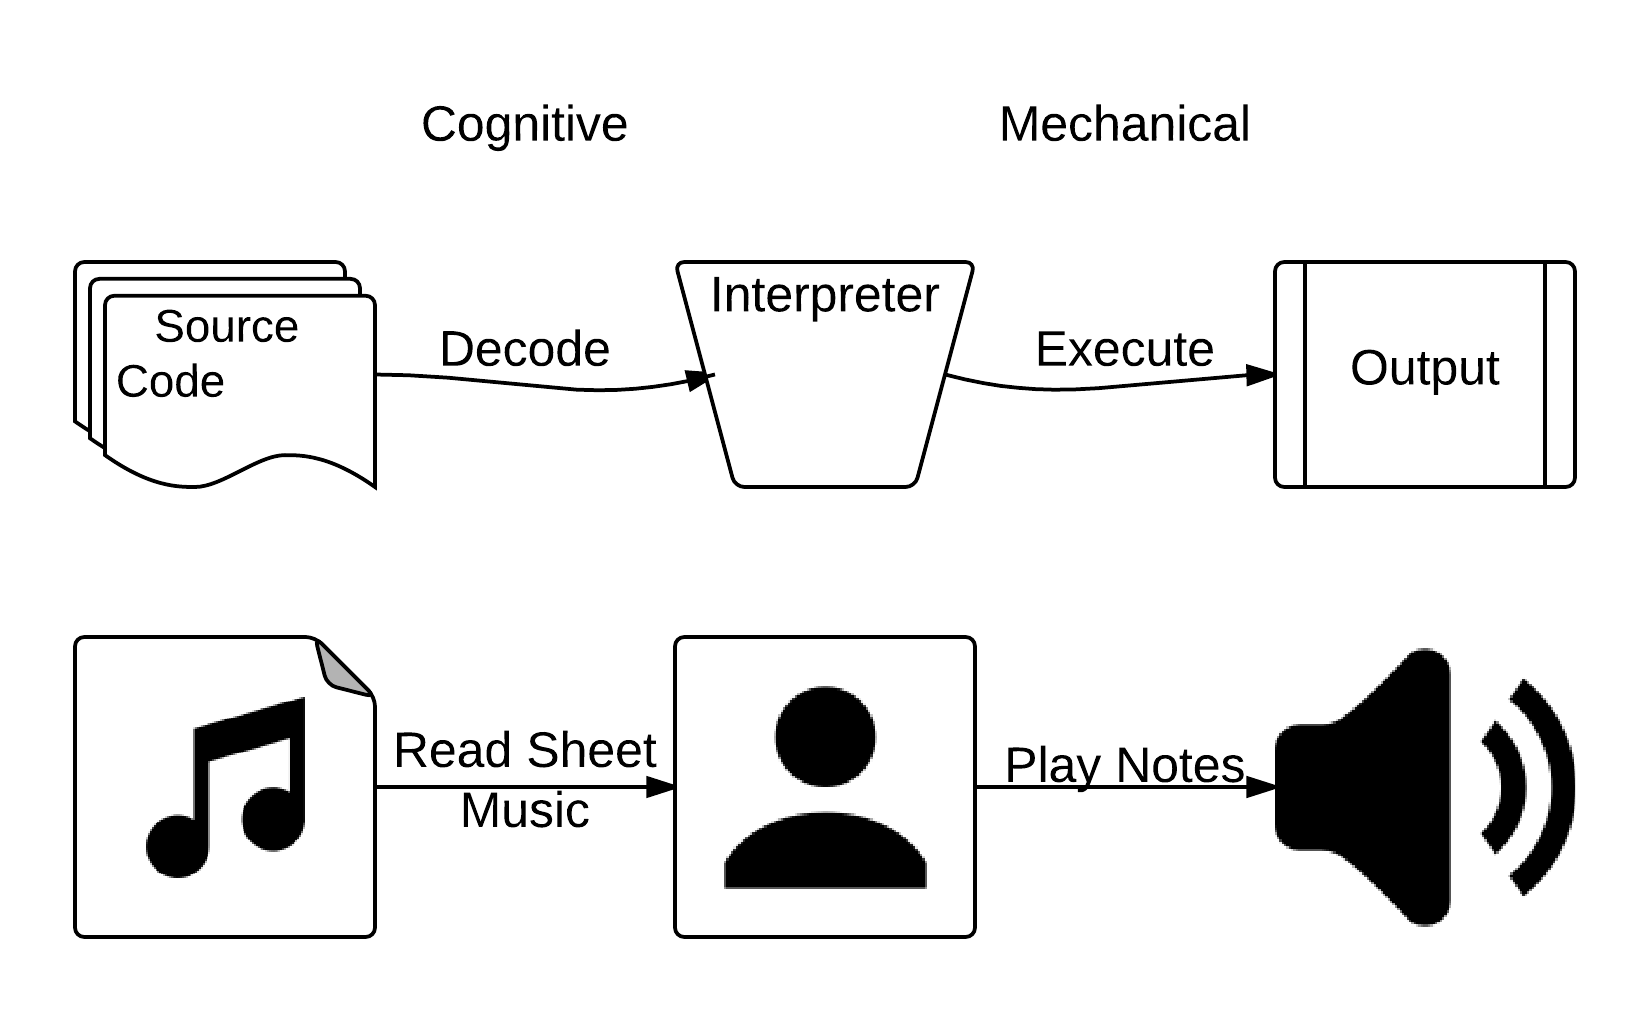
\includegraphics[width=0.47\textwidth]{CognitiveMechanical.png}
% 		\caption{The process of playing music introduces cognitive and mechanical complexities in reading and playing notes, respectively, just like interpreting high-level code into a virtual machine and executing it to produce output.}
% 		\label{image:complexities}
% \end{figure} 

\begin{figure}[ht!]
	\centering
		\caption{The process of decomposing code and music to extrapolate a conclusion.}	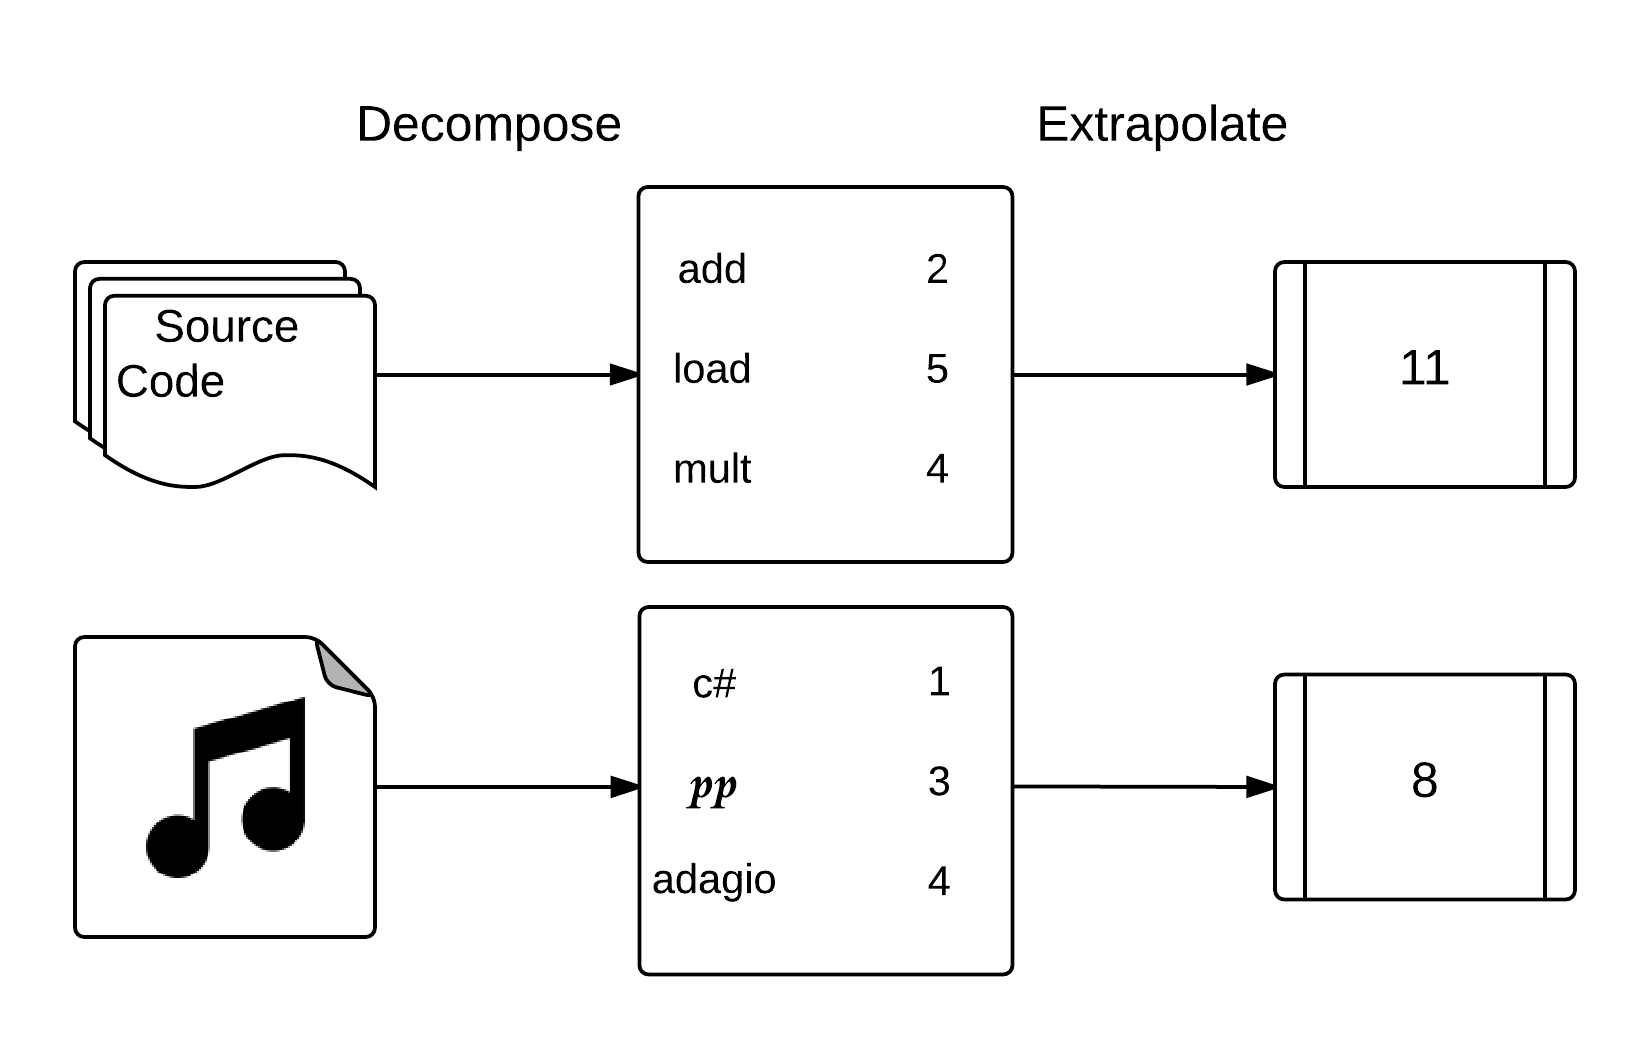
\includegraphics[width=0.8\textwidth,natwidth=1650,natheight=1050]{ComputationalThinkingAnalogy.png}
		\label{image:analogy}
\end{figure} 

Although one can draw various analogies between music and computing, the intricacy of determining the complexity of music scores is most similar to estimating program performance on different computing devices. While the same compiled program can be executed on any computing device of a given architecture, the device's processing power ultimately determines the efficiency of the resulting execution, which can vary widely. The same applies to the complexity experienced by musicians with dissimilar levels of proficiency when performing the same piece on a given instrument. Although all musicians read a piece of sheet music and understand it similarly, the complexity of playing that piece is determined by a performer's proficiency. Musiplectics aspires to blaze a trail toward objectively assessing these complexities by creating a practical computational framework that can capture the subtle nuances of musical complexity.

The solutions presented herein are instrument agnostic. Nevertheless, to realize the concept of musiplectics, the reference implementation of the computational framework targets the B$\flat$ Clarinet. This exclusive focus on clarinet is reflective of my own music performance expertise, rather than of any limitations of the presented concepts.

\section{Research Contributions} 
\label{sec:rqg}

%The overall goal of this paper is \textbf{to present a new approach to measuring the complexity of music pieces that is both objective and easy to use}.

%\item What weights would be necessary to make those grades match complexity scores (if they can be made to do so)?

% In presenting musiplectics, we aim to answer the following research questions which have guided us throughout the project:

% \begin{enumerate}
% \item What musical elements should make up the complexity of musical pieces?
% \item How should these elements factor into a complexity score?
% \item How should each element be weighted on each instrument, specifically on B$\flat$ Clarinet?
% \item What tools do musicians and educators need to access these complexity scores?
% \item Are the current grades for music competition pieces relatively correct?
% \end{enumerate}

By presenting my work, this thesis makes the following contributions:

\begin{enumerate}
\item Musiplectics, a new application of computing that encompasses automated assessment of the complexity of music scores.
\item A computational model for music complexity; it assigns base levels of difficulty to an instrument's notes and intervals, with dynamics, articulations, key signatures, and note duration serving as multipliers that increase or reduce the base difficulty.
\item Musical Complexity Scoring or MCS, a concrete realization of the musiplectics-based model above, made publicly available online for teaching and experimentation.
\item A preliminary evaluation of the model's realization, which compares MCS to commonly accepted educational level guidelines for repertoire pieces.
\item An evaluation of music Optical Character Recognition (OCR) software as a means of converting sheet music into a computer-readable MusicXML format.
\end{enumerate}

\section{Definition of Terms} 
\label{sec:terms}

Due to the nature of this research, several disciplines intersect and bring with them specific definitions and connotations for certain terms. Here I outline such terms used within this paper that may conflict with definitions used in practice by outside diciplines.

First and most obvious are the terms ``complexity'' and ``difficulty''. Throughout this thesis, complexity and difficulty are utilized interchangably to refer to the level of play required to successfully reproduce or execute a piece of music by a performer. The intent for these terms is to correlate to the measurements specified in graded works. It is most analogous to the difficulty of an olympic dive being performed, where a higher score implies a higher degree of difficulty. Similarly, these terms do not encompass the measurement for what a performer actually does (how well the dive was executed). This is not necessarily true for the definitions of complexity and difficulty within the realms of psychology or philosophy, but for the purposes of this work, they are treated as identical.

Along the same vein, here the terms mental and cognitive, as used to describe a certain component of complexity, are also used interchangably. In other disciplines mental and cognitive can separately refer somewhat analogously to affect and effect. In this thesis mental and cognitive are used in the same way to describe the components of complexity which are within a person's understanding (as in how difficult it is to simply understand exactly what a piece of music requires), as compared to mechanical or physical components (as in how difficult it is to execute the understood piece of music on a given instrument). Mental or cognitive compared to mechanical or physical is somewhat analogous to reading compared to writing.

\section{Paper Roadmap} 
\label{sec:layout}

The remainder of this thesis is structured as follows. First, Chapter \ref{sec:background} presents background information on music to provide a base line for readers. Then, Chapter \ref{sec:related} highlights related work in this field. Next, Chapter \ref{sec:scoring} explains the basic model for determining music complexity. Afterwards, Chapter \ref{sec:proof} details the proof of concept's design and details. This leads into the evaluation chapter \ref{sec:eval} which shows how I have tested this system and what preliminary results I have uncovered. Chapter \ref{sec:discus} interprets the results and discusses how the system compares to the state of the practice. Afterwards, Chapter \ref{sec:future} gives directions for future work. Finally, Chapter \ref{sec:conclu} presents my conclusions for this project.

\chapter{Background} 
\label{sec:background}
\markright{Ethan G. Holder  \hfill Chapter 2. Background \hfill}

This research is concerned with evaluating musical complexity. Music is a very specialized domain with its own unique set of concepts, terms, and conventions. Hence, for the benefit of the reader not familiar with Western music, I next present a brief refresher of the standard elements of music. The reader well-versed in this art can safely skip this chapter. Although I have striven to adhere to the standard definitions of the common musical elements, this chapter distills music theory down to the core concepts for the sake of brevity. For more advanced background information beyond what is provided here, there are many free resources available, such as MusicTheory.net \cite{MusicTheoryNet} or the Society for Music Theory \cite{SMT}.

The fundamental building block of music is the note. Notes in music are similar to words in spoken language or tokens in code. The characteristics expressed by a sound require multiple types of visual symbols to express a note. In written music, the most important characteristics of notes are pitch, duration, dynamics, and articulation. In sheet music, notes are depicted as ovals, both with and without a line (stem) and flag attached to them.

Notes are placed into measures. A measure is a uniform unit of time that breaks up a music piece into smaller segments. These smaller segments endow the piece with a repeating rhythmic emphasis, analogous to meter in poetry.

Pitch is the most salient characteristic of any note. It is the frequency of the sound wave the note produces, or how high or low a note sounds to the listener. Pitches are not continuous, but rather fall on specific discrete steps or half steps within the range of audible frequencies. 

An interval is the difference in pitch between two notes. Each interval's name encodes the distance between pitches with different levels of gradation. For example, a minor third, a perfect fourth, a major sixth, etc.

The pitch of a note can be determined from the note's vertical placement on the staff (the five horizontal lines and four spaces in between), the clef (the range of notes possible to represent on the staff), and the key signature (the pitches to be altered up or down a half step). Accidentals can also similarly alter the pitch of a note up or down by half steps; but accidentals are not applied to the entire piece, only one specific measure at a time. Both accidentals and key signatures are represented by symbols called sharps or $\sharp$, which raise the pitch a half step, flats or $\flat$, which lower the pitch a half step, and naturals or $\natural$, which undo the effect of the previously applied pitch modification. Web designers can draw an analogy from key signatures and accidentals in music to global and inline cascading style sheets (CSS) \cite{css} in web page rendering.

Another central characteristic of a note is its duration. Duration is simply the length of time a note is sustained. Although written music does not explicitly specify duration, it is inferred from the note's value (a fraction expressed by the note's stem and flags), the time signature (how many beats are in a measure and what fraction of a whole note gets a beat), and the tempo (how many beats are played in a given time frame).

For example, the value of a quarter note is $1/4^{th}$ that of a whole note. In three four time, the first number says there are three beats in a measure, and the second number says that a quarter note receives one beat in a measure. If the tempo is 120 bpm (beats per minute), then this example measure would last exactly 1.5 seconds (3 beats in a measure / (120 beats per minute / 60 seconds/minute)).

Dynamics refers to the volume of notes. Dynamics are specified with different Italian words, such as piano (quiet), forte (loud), and mezzo (medium), expressed by letter \textbf{p}, \textbf{f}, and \textbf{m}, respectively. Composer combine these letters to express a wide variety of dynamic levels, typically ranging from \textbf{ppp} (pianississimo, meaning very, very quiet) to \textbf{fff} (fortississimo, meaning very, very loud). There are also markings for gradually changing dynamics to louder (crescendo) or softer (decrescendo or alternatively diminuendo) that look like elongated greater than or less than symbols below the staff.

Articulation is how a note is played and linked to subsequent notes. The simplest analogy for articulations are how different letters or sounds are formed and connected in spoken language. For example, speaking ``ta'' and ``la'' have the same ``a'' sound once held out, but their initial articulations are different because the ``t'' and ``l'' sounds are uttered differently. There are many different articulations, but the main ones utilized in this work are as follows:

\begin{itemize}
\item Accent or $>$, which means to play the note louder than those around it.
\item Staccato or $\cdot$, which means to play the note shorter than its full value, cutting it off early.
\item Tenuto or -- , which means to play the note slightly longer than its full value, in a connected manner to the following note.
\item Marcato (a strong accent) or $\wedge$, which means to play the note much louder than those around it, more than an accent.
\item Slur or $\smile$, which means to separate only the first note, connecting all the following notes together.
\end{itemize}

Although musical notation possesses additional advanced characteristics, including timbre, further articulations, and elaborate music markings, we did not find these advanced symbols as common enough to be useful to consider in a general complexity model. When writing music, composers combine the concepts above to express the desired artistic impression the composition is intended to make on the listener. Hence, it is hard to distinguish which notational concept is more important than the other for artistic expression. Nevertheless, we have found the subset presented above as absolutely essential to realizing the ideas behind musiplectics.

\chapter{Related Work} 
\label{sec:related}
\markright{Ethan G. Holder  \hfill Chapter 3. Related Work \hfill}

Multiple prior research efforts study various facets of music. Although relatively few works concretely focus on analyzing music complexity \ref{sec:relcom}, tangential studies into scanning and searching music \ref{sec:relscan} as well as classifying music \ref{sec:relclass} represent related research efforts. Each has tangible ties to this work's objectives, albeit some at a more abstract level than others.

%Cover any related work in the field and differentiate this project.

\section{Complexity Analysis}
\label{sec:relcom}

The most relevant works to musiplectics are those that also seek to analyze the complexity of music in some way. A representative example is presented in reference \cite{Chiu2012}. This work seeks to automatically generate or predict the difficulty of a piano music piece. The authors apply regression theory over a set of features that cause difficulties for that specific instrument. Musiplectics leverages similar musical concepts to build up an aggregate measure of difficulty or complexity. However, my approach has a wider range of applicability, both in terms of musical instruments and playing proficiency, as well as portability, by embracing uniform types of complexity parameters. In other words complexity parameters in musiplectics encompass the cognitive and mechanical complexities for a given instrument. So all instruments have the same types of complexity parameters, which may take upon vastly different values.

Similar to \cite{Chiu2012}, \cite{Heijink2002} studies the complexity of playing guitar. Their work extracts features that determine difficulty when playing guitar. However, their focus lies more on the mechanical difficulties specifically associated with that instrument rather than broad ranging complexities of playing music on any instrument. Musiplectics also takes into account the playing proficiency of the player at hand.

Another related approach lies in \cite{Liou2010}. The authors analyze the complexity of the rhythmic components of various pieces of music. They utilize the L-system to breakdown the rhythm of a piece into a tree structure and then apply tree analysis algorithms to generate a score. Although musiplectics avoids complex algorithms for examining the rhythmic structure of a piece, it considers a full array of the elements of music scores rather than simply rhythm alone.

State organizations, such as \cite{VBODA} in Virginia and \cite{NYSSMA} in New York as well as others, similarly analyze music scores by hand, an activity which we hope to automate. These organizations govern K-12 schools in their respective states. They also list music pieces and their respective difficulty grades for district, regional, or state competitions for each K-12 grade level. Other organizations, such as the Royal Conservatory Music Development Program \cite{RoyalSyllabus}, offer similar pieces and respective grades as part of their level requirements and assessment regulations. Unlike state organizations, Royal Conservatory publishes their pieces and scores to the public, a provision that enables leveraging them in evaluating this work.

The difficulty grading schemes in both types of organizations are analogous to the complexity of the piece, except that in these organizations pieces are graded subjectively by a group of people rather than a uniform algorithm. Additionally, the grades are typically listed as integer values between 1 and 10, thus lacking a sufficient level of granularity to express nuanced differences between musical pieces.

Further past works have specifically studied the complexity of music as experienced by listeners or observers. These works show great insights into defining complexity and in fact utilize very similar music elements as representative features to determine overall complexity. For instance, \cite{madsen2006music} relies on note pitches, intervals, and durations of notes as features on pieces of MIDI formatted music to determine the complexity experienced by listeners. Similarly, \cite{streich2006automatic} presents an entire Ph. D. thesis on characterizing the complexity of music from the viewpoint of the listener. Other works have specifically utilized listener complexity in related studies \cite{Heyduk1975} \cite{parry2004musical} \cite{mauch2011structural} \cite{orr2001relationship} \cite{williams2005effect} \cite{burke1990musical} \cite{north1999can} \cite{steck1975preference}.

Several related works from \cite{streich2006automatic} also formally define what complexity is in terms of listeners and what information can be gathered from it as a property of music \cite{edmonds1995complexity} \cite{pressing1999cognitive} \cite{scheirer2000perceived}. While this thesis focuses on the complexity experienced by performers, such related works all provide a basis to build upon \cite{Knuth:1984:CS:358027.358042}. Future work could seek to compare the complexity experienced by listeners or observers to that of the performer to see what similarities (if any) arise.

\section{Music Scan \& Search}
\label{sec:relscan}

One area of research tangential to analyzing music complexity is scanning and searching for music. The overlap lies chiefly in the end use cases in both areas of research. Educators, performers, and other stakeholders, all find themselves needing to efficiently locate musical pieces that meet their respective requirements. Providing a complexity score is one means to improve the efficiency of searching for new music, since users can see complexity at a glance or even search by complexity to find a piece to prepare. \cite{Byrd2001} gives many reasons for why this is necessary, but there is a whole body of research related to music information retrieval that deals with similar problems \cite{downie2003music} \cite{casey2008content}.

Another area of overlap between musiplectics and music scanning is in translation. From a high-level, reading in any form of music and writing out a related, different form is essentially translation, an area which I have previously explored in some depth \cite{holder2013cloudASE} \cite{holder2013cloudSPLASH} \cite{holder2014native}. There are many research efforts to translate forms of music into other languages or versions.

An especially interesting effort in this regard is \cite{Allali2009}. The authors work to convert polyphonic music (music with several simultaneous notes on one or several instruments, such as a band playing together in harmony or one person playing piano or guitar for instance) into equivalent monophonic music. Their end goal is to reduce a large, expressive format to a more simple one for comparing pieces during a lookup. The reduction in complexity of chords down to single notes represents an interesting approach that could be leveraged with musiplectics, so as to generate a potentially less complex version of a given piece.

\section{Music Classification}
\label{sec:relclass}

Music classification presents another area of potential research overlap. Much research has previously dealt with using computers to understand music and thus classify into various genres. While the efforts of music classification are not the same as determining complexity, the approaches taken to classify certain pieces via machine learning and statistical methods are important, because they present means of automatically analyzing music. At some point musiplectics could potentially apply similar machine learning concepts to interpret what makes music complex (rather than decomposing music scores into individual elements and calculating their summary complexity) as well as leverage genre classification as another source of potential complexity.

Cuthbert, Friza, and Friedland \cite{Cuthbert2011} for example focused heavily on using machine learning to classify different types of music. The authors can extract multiple features from a variety of input types and apply their theorem to successfully classify the genre of several inputs.

Similarly, \cite{Cataltepe2007} proposes an approach to classifying music files in MIDI format specifically. The authors form an approximation of the Kolmogorov distance using the normalized compression distance between approximate string representations. They use this approximation as the main feature to classify numerous music files.

\chapter{Computational Model for Music Complexity} 
\label{sec:scoring}
\markright{Ethan G. Holder  \hfill Chapter 4. Computational Model for Music Complexity \hfill}

In Chapter \ref{sec:background} above, I discussed several fundamental music concepts. These concepts serve as the baseline elements that factor into the complexity score. 

The most straightforward approach to calculating an overall score is to assign whole number weights to each element perceived to be especially important (i.e., notes, intervals, dynamics, articulations, key signatures, and note durations) and add all the weights up. This scheme, however viable, fails to adequately reflect the experience of playing music. At their core, notes and intervals present distinct difficulties on their own, whereas dynamics, articulations, key signatures, and note durations only modify those difficulties. For instance, a small interval may seem easy on its own, but with changing dynamics, with differing articulations, in a strange key, or at a high tempo, that interval could become much more difficult.

Hence, a more authentic approach to calculating an overall score is to only assign whole numbers weights to notes and intervals. These are still counted and summed up into a final score. However, dynamics, articulations, key signatures, and note durations become multipliers onto notes and intervals. Each dynamic, articulation, and key signature thus receives a multiplier weight that is a decimal (typically between 0 and 2). Those multipliers are applied to every occurrence of a note or interval.

Note duration is factored into the score as an average over all notes. The total amount of notes and associated duration in seconds is calculated at the end and applied as its own multiplier. The more notes in a given span of time, the higher the multiplier becomes.

This scheme captures the concept previously envisioned that makes duration add to overall complexity, except in the extreme case of playing excessively long notes. In cases of wind instruments, such as the main target of B$\flat$ Clarinet, holding notes out for long durations may possess its own difficulty in providing adequate breath support, rather than the difficulties of changing finger positions and embouchure quickly.

Thus, the model adapts the note duration multiplier to be a multiplicative or fractional difference from one. If the average of notes per second in the piece is 1.5, then the multiplier remains 1.5. However, in the case of many long notes, the average of notes per second might be something closer to 0.5. In this case (when the average is less than 1), the fraction becomes its reciprocal, 2 in the example.

Users cannot directly change this parameter as it is built into the model. However, they can still influence the degree to which this parameter affects the overall score. To that end, the user can parameterize note durations with a multiplier value that increases or reduces the impact of the note duration parameter. For the cases when the user is content with the built-in setting, the model applies the default value of 1.

\chapter{Proof of Concept} 
\label{sec:proof}
\markright{Ethan G. Holder  \hfill Chapter 5. Proof of Concept \hfill}

In \ref{sec:design}, I outline the basic software design of the proof of concept. Next, I provide some highlights of the extensible architecture in \ref{sec:highlights}. Then, I describe the full details of the overall implementation in \ref{sec:details}.

\section{Design Overview} 
\label{sec:design}

The complexity model presented above outlines the basic functionality of the approach. Nevertheless, the implementation's complete control flow involves several steps. The extended control flow based on the model can be seen in Figure \ref{image:flow}.

\begin{figure}[ht!]
	\centering
		\caption{The extended control flow showing the model forming the complexity score.}
		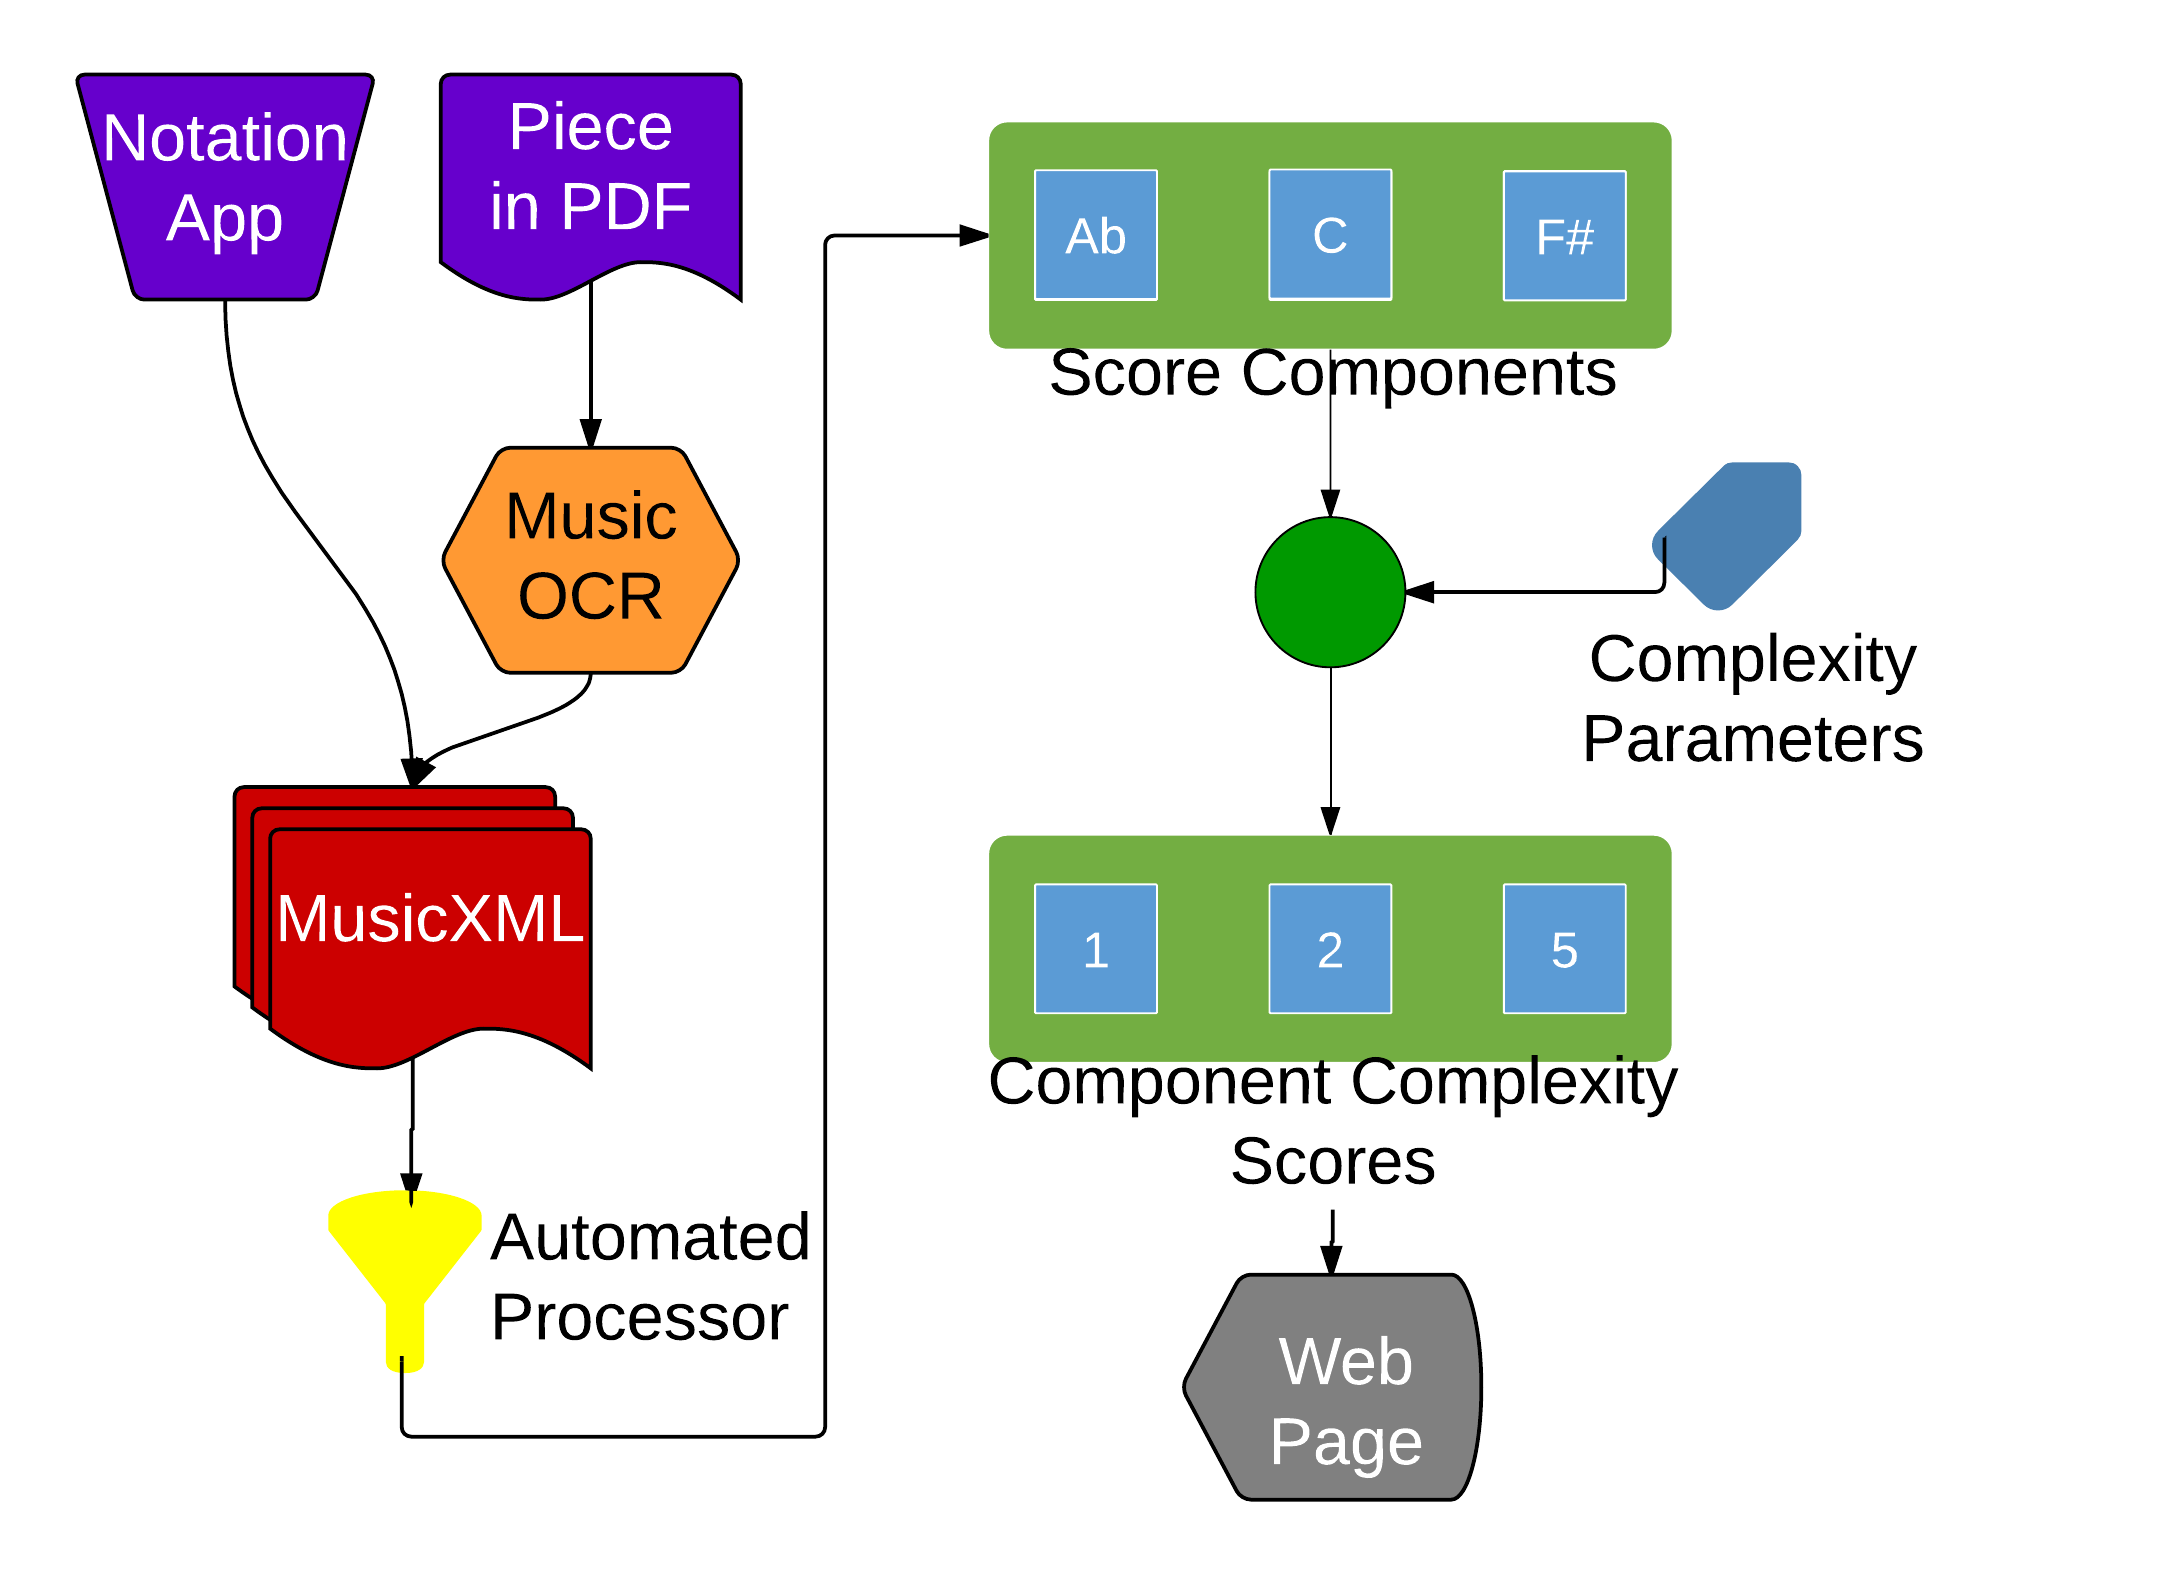
\includegraphics[width=0.8\textwidth]{JoinedCropped.png}
		\label{image:flow}
\end{figure}

From the top left, one can see the inputs to our a musiplectics system are Notation Apps and Pieces in PDF format. Many common notation applications, such as Finale Notepad \cite{FinaleNotepad} and Sibelius \cite{Sibelius}, support a universal format called MusicXML \cite{MusicXML} \cite{Good2001}. MusicXML files can be imported, edited, and output back to MusicXML or other proprietary formats. MusicXML is the underlying representation on which the reference implementation operates.

Alternatively, the system can be extended to work directly with music pieces in PDF format. It can accept PDF files and transform them into their MusicXML representation, by means of music OCR (Optical Character Recognition) software. The reference implementation relies on free software from Audiveris \cite{Audiveris} currently, but it could equivalently utilize other off-the-shelf OCR applications.

Once the MusicXML representation of the piece is obtained, the automated processor then takes it as an input. The processor computes the complexity score by going through a sequence of steps. First, it parses the piece to extract individual music elements to be analyzed. Then, it looks up the weights for each element as specified by the complexity parameterization.

Recall that this system can be parameterized with different complexity weights to reflect dissimilar levels of per-instrument playing proficiency. Currently, these weights are specified in an xml file to facilitate tool integration. Because the weights are meant to be decided on by music experts, the design foresees the creation of visual editors to specify this information. These editors can easily save their inputs in some xml format. Similarly, individual users could create their own file representing their own personal weights and apply the system in the same manner. In the proof of concept, I experimented with 5 different sets of weights, which represent proficiency levels that range from that of a beginner up to a trained professional.

Using the specified weights, the system calculates the complexity by tallying up the difficulty values of each individual type of element, computed separately during a single pass over the structure. The final piece of functionality presents the calculated complexity in a user friendly fashion. To that end the system uses a web-based interface with specialized javascript libraries.

\section{Architecture Highlights} 
\label{sec:highlights}

One key design feature is ease of extendability at each level. Any application that generates valid MusicXML files can feasibly provide input to this system. Furthermore, the overall process can be extended if other applications can generate the piece of music in PDF form or some intermediate that can be represented in PDF or MusicXML.

The system itself can be extended to operate only on specific selections of pieces or on batches of multiple pieces if necessary (thus showing the complexity of an entire performance). Additionally, the parameters that determine complexity can easily be changed on the fly based on future refinements. This provision enables individual performers or groups to set their own complexity levels to find a score even more relevant to their playing style.

Beyond the extension to the current process, the system can be easily scaled up to operate for many users on many music pieces. The current complexity parameters can be quickly substituted with an external database in MySQL \cite{mysql}. Additionally, libraries of MusicXML pieces along with user uploaded files can easily replace pre-selected pieces currently available.

Even the backend software itself can be extended and modified in the future with relative ease. MusicXML files are parsed with heavy reliance on the Visitor Design Pattern \cite{gamma1994design} and judicious overloading \cite{bloch2008effective}. In doing so the intricacies and redundancies of MusicXML are effectively abstracted away, and future additions to the model are easily accommodated.

Finally, the javascript libraries used on the frontend naturally facilitate creating a mobile-friendly web interface. While mobile experiences have not yet been fully optimized, they are still readily available even now. Furthermore, it would be straightforward to extend this interface into a mobile app itself by utilizing past translational research \cite{holder2013cloudSPLASH} \cite{holder2013cloudASE} or PhoneGap \cite{phonegapBook} \cite{phonegapArticle}.


%Talk about the high level approach for how this works in terms of the musical elements defined in the background section earlier.

\section{Implementation Details} 
\label{sec:details}

The reference implementation spans several different code bases, most notably the automated processor backend and the web UI frontend. This style of two-tier architecture is common in both web and mobile applications. Figure \ref{image:architecture} shows a diagram detailing the specific architecture for the reference implementation and showing how the frontend and backend pieces interact.

As shown, when a user first requests a complexity score from the frontend interface, that request is formatted as AJAX \cite{garrett2005ajax} and sent to the backend web server. The physical server receives the request and routes it to the appropriate running service (in this case, the backend). Once the backend receives the request, it fetches the complexity parameters and the piece in MusicXML format specified by the user. Then, the backend code generates the complexity score as discussed previously in the design overview. It formats the complexity score as well as some related data (the most complex measure number and form, note complexity including associated multipliers, and interval complexity including associated multipliers) for each part within the piece of music into JSON \cite{crockford2006application} data before sending the response back to the frontend. When the frontend receives the asynchronous response, it parses the JSON data and displays the complexity score and related data in graphical format.

\begin{figure}[ht!]
	\centering
		\caption{The architecture and flow of the backend and frontend code bases.}
		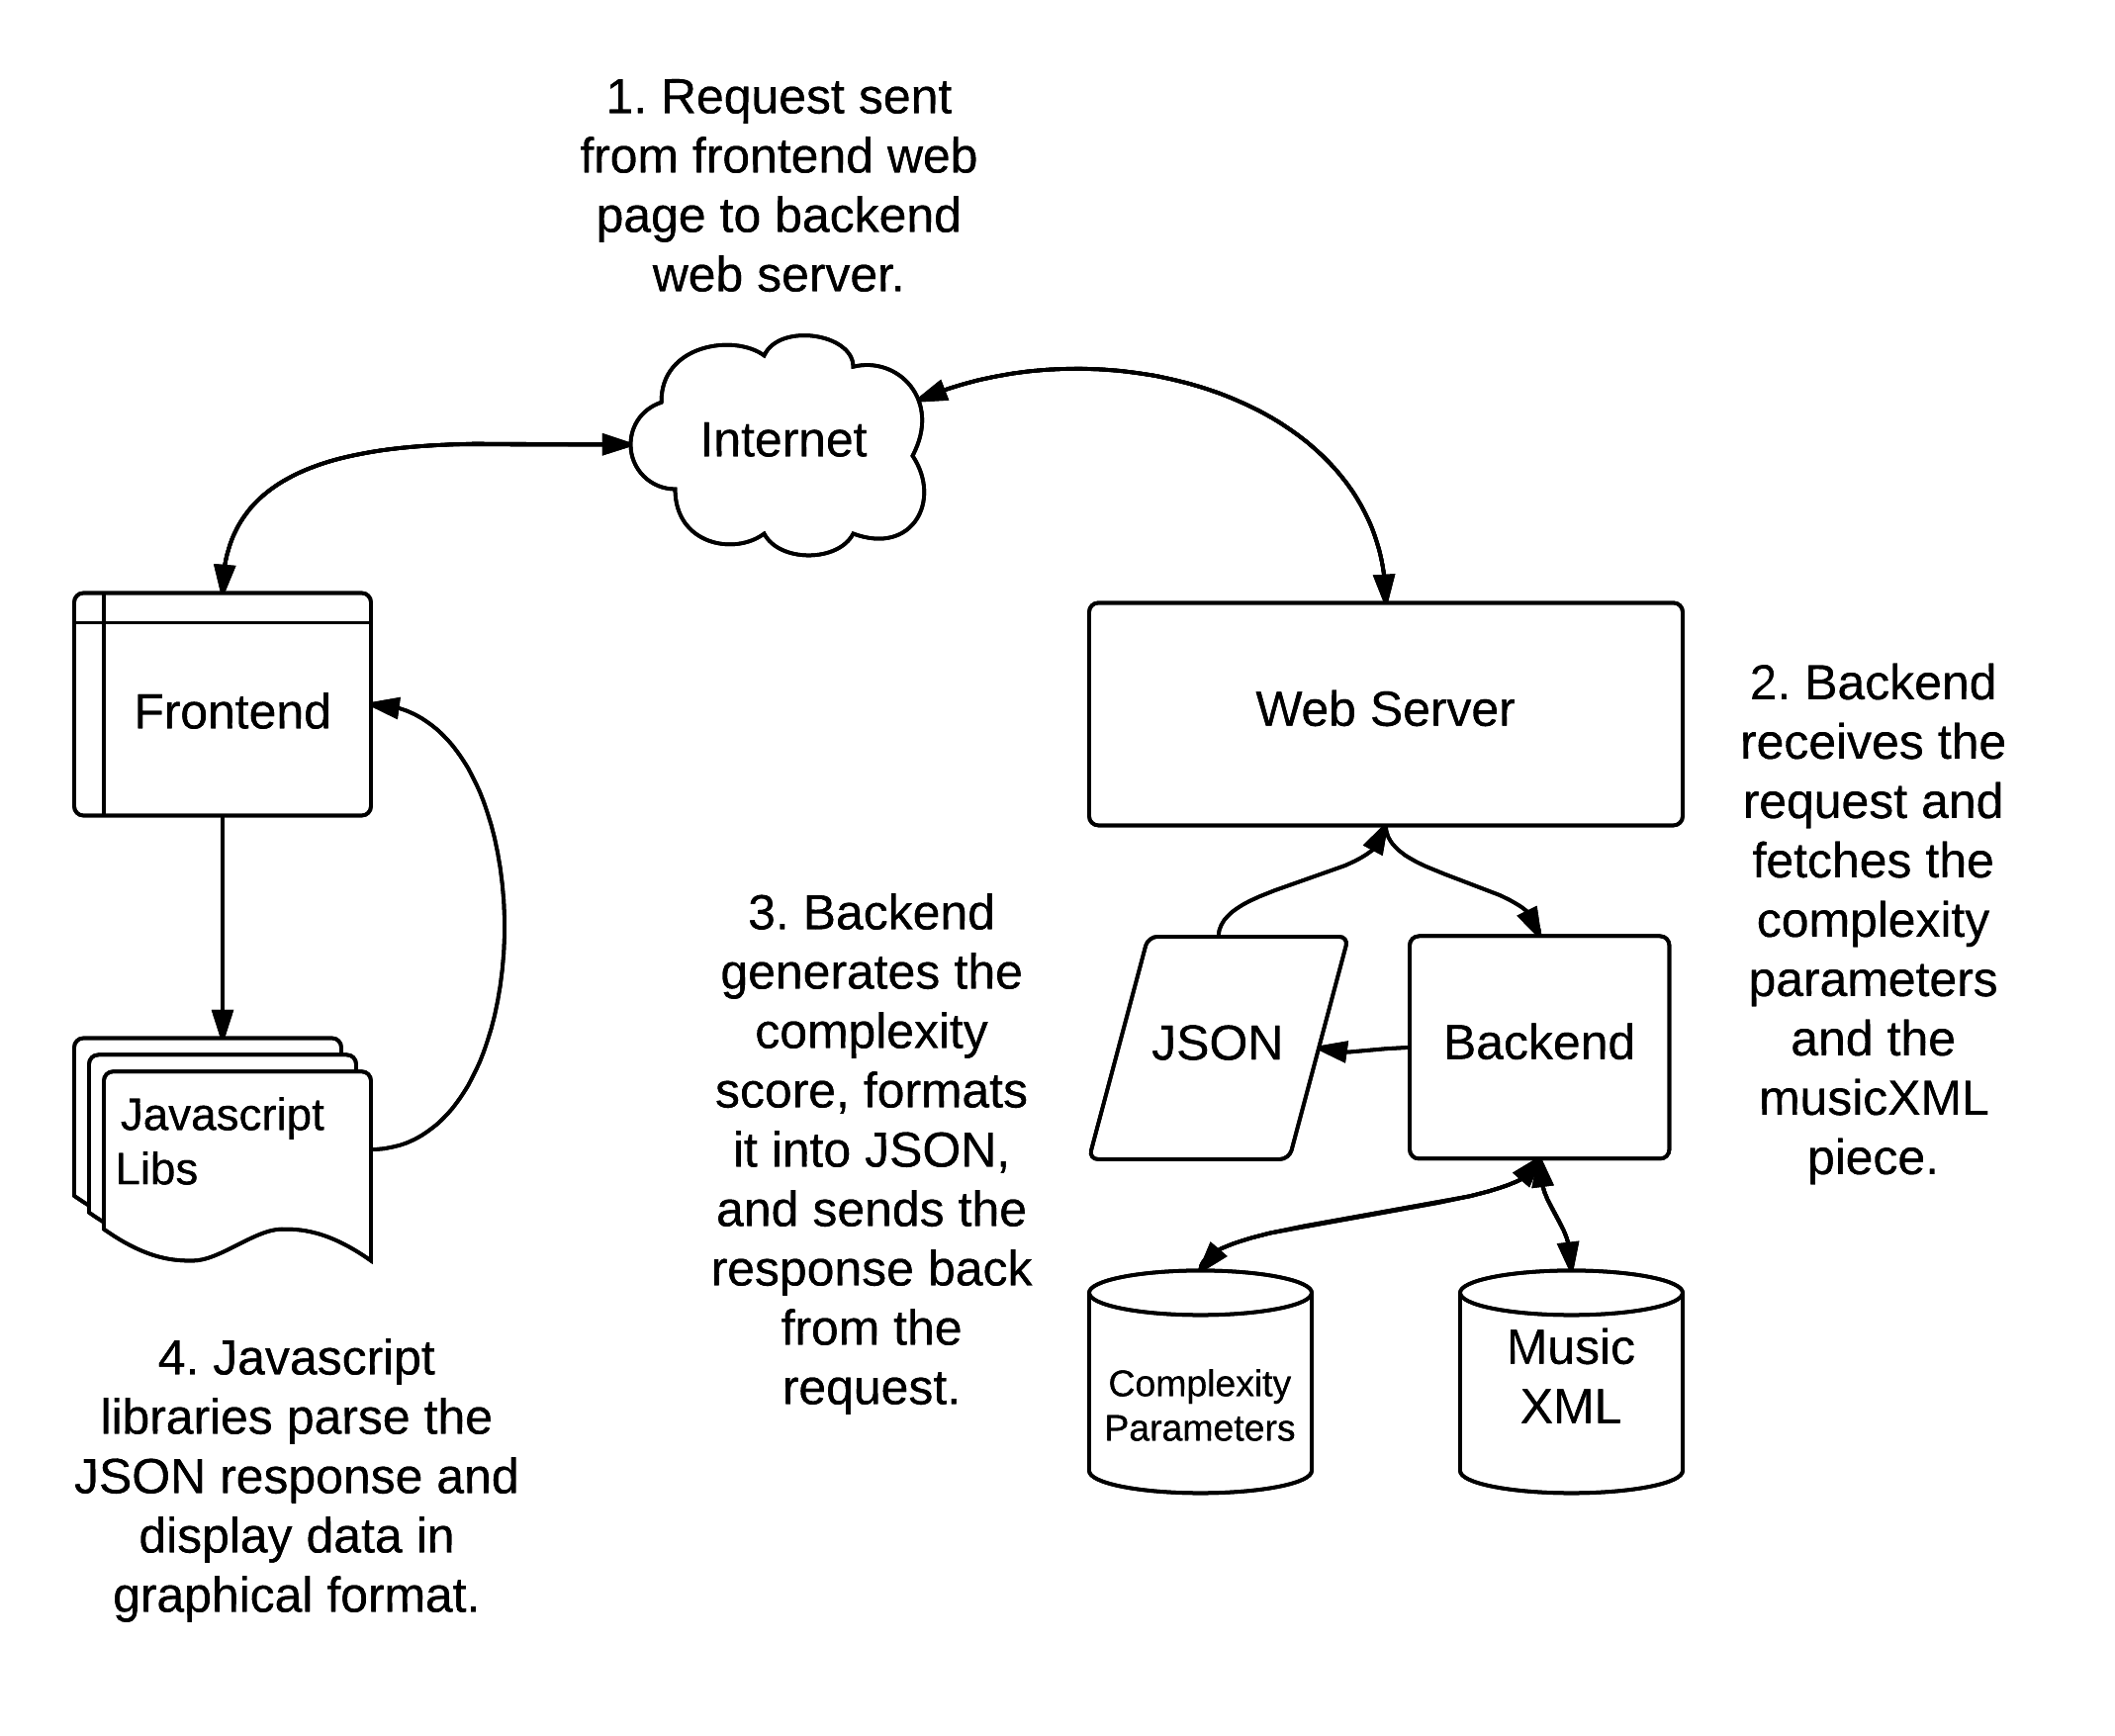
\includegraphics[width=0.8\textwidth]{Architecture.png}
		\label{image:architecture}
\end{figure}

The backend code is written in Java \cite{java} and spans 5137 source lines of code (SLOC) \cite{nguyen2007sloc}. I've utilized the Apache Xerces 2.11.0 library for parsing xml files \cite{XMLAPI} and the JSON Simple 1.1.1 library \cite{JSONAPI} for constructing JSON \cite{crockford2006application} to pass along to the frontend. This Java backend is compiled and bundled up as an executable. It is then run via command line interface, specifying the complexity parameters and MusicXML to run against.

As mentioned previously, the backend utilizes the visitor pattern heavily when processing the MusicXML file. The visitor pattern eases the handling of the intricacies and redundancies of MusicXML by allowing different operations to be defined on the classes of elements present within MusicXML. It also abstracts away the requirement for a specific MusicXML structure.

The simplest way to demonstrate this abstraction is through the placement of specific xml elements within the MusicXML file. For instance, the elements ``sound'' and ``direction-type'' typically hold new ``tempo'' or ``dynamics'' elements as children, respectively. Obviously, tempo and dynamics must be tracked as part of the complexity score so their elements must be tracked, thus their parent elements must be tracked as well. However, ``sound'' and ``direction-type'' elements do not always appear in the same location within the MusicXML file. Both can occur as a child of a ``direction'' element or as a child of a ``measure'' element. Therefore, the system needs to be robust enough to encounter these types of elements at varying depths within the MusicXML's tree structure. Visitor pattern succinctly accomplishes that goal.

The compiled backend code is currently deployed on a Unix-based Mac Mini \cite{macmini} running OS X Mavericks (version 10.9.1) \cite{osx}. A lightweight Apache server \cite{apacheServ} hosts the files and runs some limited PHP to facilitate easy communication between the frontend and backend portions. AJAX requests \cite{garrett2005ajax} are sent to the backend and JSON response text is sent back in the current implementation.

The frontend code is written in Javascript, HTML, and CSS and spans 3061 SLOC \cite{nguyen2007sloc}. To minimize the amount of hand-written code, the implementation makes use of numerous industry-standard libraries, including jQuery 2.1.0 \cite{jQuery}, Bootstrap 3.3.4 \cite{Bootstrap}, Datatables 1.10.5 \cite{DataTables}, D3 3.5.5 \cite{D3}, and VexFlow 1.2.27 \cite{VexFlow}. These libraries span various standard facets of system implementation, making it possible to focus on the novel, research-related issues of musiplectics when creating the proof of concept.

Both the frontend and backend as currently implemented are publicly available on GitHub \cite{GithubMusicScoring} along with instructions as to how to set them up personally. The site also features links to the currently deployed version.\footnote{The current version is deployed at \url{http://mickey.cs.vt.edu/}}

\chapter{Evaluation} 
\label{sec:eval}
\markright{Ethan G. Holder  \hfill Chapter 6. Evaluation \hfill}

The goal of this evaluation is to demonstrate that the reference implementation of musiplectics can be a useful tool for music educators. To that end, the system was run with different parameterizations on a set of music scores, used in educational settings. Music educators have also ranked these same scores by hand, producing a baseline for comparison. As expected, even though the general trends reported by the tool corresponds to that provided by music educators, some outliers were also observed. Some pieces turned out to have been much more complex on the relative scale than the pieces immediately preceding and following them in the rankings. These discrepancies can be explained either by immaturities of the implementation or by inaccuracies of ranking of music scores by hand. It is easy to overlook some really complex parts in the middle of a score when trying to assess its suitability for a given playing proficiency. While an automated tool analyzes scores in their entirety, producing the results based on an exhaustive analysis of each and every element.

I first specify the complexity parameters used in the experiments in \ref{sec:settings}. Then, I unveil the strategies one can follow to obtain the settings that represent a consensus among musicians in \ref{sec:survey}. Next, I describe the test pieces selected in \ref{sec:pieces}. Finally, I discuss the accuracy of the OCR program tested for suitability in musiplectics in \ref{sec:ocr}.

%Describe the preliminary settings used to score pieces based on clarinet and how we plan to refine them. Also talk about usability

\section{Clarinet Complexity Parameterization} 
\label{sec:settings}

Chapter \ref{sec:scoring} above explains the rationale behind complexity parameters. In particular, it differentiates between parameters, expressed as whole number weights and those which are decimal number multipliers. In that presentation, the parameters were not linked to any particular instrument. By contrast, in this Section, I discuss their specific application for a specific instrument, the B$\flat$ Clarinet.

I decided to focus specifically on the clarinet, because it exhibits many forms of complexity and relates to many similar woodwind and brass instruments. Additionally, my own musical expertise favors this instrument above all others, making it possible to define my own complexity parameters with confidence and not requiring external confirmation.

The initial complexity settings for B$\flat$ Clarinet were for beginners. Based on these values, complexity settings for other levels of B$\flat$ Clarinet were later adapted, but those levels largely changed only the associated weights. Because only the beginner settings were utilized in the tests, they are the only ones discussed below.

Note complexities were broken up into the ranges and assigned weights, as shown in Table \ref{table:notes}. Intervals were similarly broken up further and assigned weights, as shown in Table \ref{table:intervals}.  

\begin{table}[t]
	\centering
	\caption{Note ranges and weights for beginner B$\flat$ Clarinet.}
    \begin{tabular}{| l | l |}
        \hline
        Note Range & Weight \\ \hline
        G3-G$\sharp$4 & 1 \\ \hline
        A4 & 2 \\ \hline
        B$\flat$4-C5 & 5 \\ \hline
        $\geq$ C$\sharp$5 & 10 \\
        \hline
    \end{tabular}
	\label{table:notes}
\end{table}

\begin{table}[t]
	\centering
	\caption{Intervals, note ranges, and weights for beginner B$\flat$ Clarinet.}
    \begin{tabular}{| l | l | l | l |}
        \hline
        Interval & Low Range & High Range & Weight \\ \hline
        Unison & Anywhere & Anywhere & 1 \\ \hline
        Second & G3-G$\sharp$4 & G3-G$\sharp$4 & 2 \\ \hline
        Third & G3-G$\sharp$4 & G3-G$\sharp$4 & 3 \\ \hline
        Fourth & G3-G$\sharp$4 & G3-G$\sharp$4 & 4 \\ \hline
        Fifth & G3-G$\sharp$4 & G3-G$\sharp$4 & 5 \\ \hline
        Any & G3-G$\sharp$4 & A4-C5 & 8 \\ \hline
        Any & A4-C5 & $\geq$ C$\sharp$5 & 10 \\ \hline
        Sixth & Anywhere & Anywhere & 9 \\ \hline
        Seventh & Anywhere & Anywhere & 9 \\ \hline
        Octave & Anywhere & Anywhere & 9 \\ \hline
        $>$ Octave & Anywhere & Anywhere & 10 \\
        \hline
    \end{tabular}
	\label{table:intervals}
\end{table}

Dynamics and articulations were specified for those specific types mentioned previously in Chapter \ref{sec:background}. Their weights can be found in Tables \ref{table:dynamics} and \ref{table:articulations}, respectively. Unlike dynamics and articulations, all possible major key signatures are specified with weights and shown in Table \ref{table:key}. Finally, the note duration modifier is kept at 1.0, so the note duration modifier works exactly as specified in \ref{sec:scoring}.

\begin{table}
	\centering
	\caption{Dynamics and weights for beginner B$\flat$ Clarinet.}
	\label{table:dynamics}
    \begin{tabular}{| l | l | l |}
        \hline
        Dynamic & Abbreviation & Weight \\ \hline
        mezzo forte & mf & 1.0 \\ \hline
        mezzo piano & mp & 1.0 \\ \hline
        forte & f & 1.1 \\ \hline
        fortissimo & ff & 1.2 \\ \hline
        piano & p & 1.3 \\ \hline
        pianissimo & pp & 1.5 \\
        \hline
    \end{tabular}
\end{table}

\begin{table}
	\centering
	\caption{Articulations and weights for beginner B$\flat$ Clarinet.}
    \begin{tabular}{| l | l |}
        \hline
        Articulation & Weight \\ \hline
        Slur & 0.5 \\ \hline
        Normal/None & 1.0 \\ \hline
        Accent & 1.1 \\ \hline
        Staccato & 1.2 \\ \hline
        Tenuto & 1.2 \\ \hline
        Marcato (Strong Accent) & 1.4 \\
        \hline
    \end{tabular}
	\label{table:articulations}
\end{table}

\begin{table}
	\centering
	\caption{The major key signatures and weights for beginner B$\flat$ Clarinet.}
    \begin{tabular}{| l | l | l |}
        \hline
        Key Signature & Sharps/Flats & Weight \\ \hline
        C & None & 1.0 \\ \hline
        G & F$\sharp$ & 1.1 \\ \hline 
        D & F$\sharp$, C$\sharp$ & 1.1 \\ \hline
        A & F$\sharp$, C$\sharp$, G$\sharp$ & 1.2 \\ \hline
        E & F$\sharp$, C$\sharp$, G$\sharp$, D$\sharp$ & 1.3 \\ \hline
        B & F$\sharp$, C$\sharp$, G$\sharp$, D$\sharp$, A$\sharp$ & 1.4 \\ \hline
        F$\sharp$ & F$\sharp$, C$\sharp$, G$\sharp$, D$\sharp$, A$\sharp$, E$\sharp$ & 1.5 \\ \hline
        C$\sharp$ & F$\sharp$, C$\sharp$, G$\sharp$, D$\sharp$, A$\sharp$, E$\sharp$, B$\sharp$ & 1.6 \\ \hline
        F & B$\flat$ & 1.1 \\ \hline
        B$\flat$ & B$\flat$, E$\flat$ & 1.1 \\ \hline
        E$\flat$ & B$\flat$, E$\flat$, A$\flat$ & 1.2 \\ \hline
        A$\flat$ & B$\flat$, E$\flat$, A$\flat$, D$\flat$ & 1.3 \\ \hline
        D$\flat$ & B$\flat$, E$\flat$, A$\flat$, D$\flat$, G$\flat$ & 1.4 \\ \hline
        G$\flat$ & B$\flat$, E$\flat$, A$\flat$, D$\flat$, G$\flat$, C$\flat$ & 1.5 \\ \hline
        C$\flat$ & B$\flat$, E$\flat$, A$\flat$, D$\flat$, G$\flat$, C$\flat$, F$\flat$ & 1.6 \\
        \hline
    \end{tabular}
	\label{table:key}
\end{table}



\section{External Survey} 
\label{sec:survey}

Although the complexity parameterization presented in \ref{sec:settings} may be accurate, one would not be able to validate them empirically, as they reflect one's subjective personal experiences and beliefs. However, musiplectics embraces this subjectivity, enabling individual musicians to specify the parameterizations that reflect their own individual understanding of their own or their students' proficiency.

As a logical consequence of the previous observation, it would be equally impossible to empirically validate the ``correctness'' of the computed complexity score of an analyzed piece. However, if stakeholders in a score can generally agree on its relative complexity, the resulting consensus can serve as a viable form of validation.

Based on this assumption, experts, musicians, and educators seem to have a vested stake in the results of these complexity scores. Therefore, I've begun to survey those related to B$\flat$ Clarinet in an effort to ascertain their opinions. In the survey I ask simple questions about the complexity parameters already established, both how the parameters are implemented and the weights assigned to each. Once a statistically significant consensus has been reached or some threshold of responses have been given, the results of the survey will become the new complexity parameters. At the time of writing, neither condition has been met so my own parameters are in use, but it is important to note that I am striving to find an amicable means of determining these parameters.

\section{Graded Music Pieces for Comparison}
\label{sec:pieces}

Based on the 2014 syllabus for B$\flat$ Clarinet available from Royal Conservatory \cite{RoyalSyllabus}, I selected 2-4 pieces for each grade, 1-10. The pieces were chosen based on availability, so as to minimize the amount of companion book or subscription purchases required. In whole 32 pieces are used for the main comparison: 10 from Standard of Excellence \cite{Standard}, 7 from Clarinet Solos \cite{Solos}, 4 from Concert and Contest Collection \cite{Concert}, and 11 publicly available on IMSLP \cite{IMSLP}. Each of these is listed with its author and grade in Table \ref{table:pieces}. These pieces are translated into MusicXML using the OCR process and subsequently passed through my system to obtain a complexity score for each.

\begin{table}[ht!]
	\centering
	\caption{The works from Royal Conservatory chosen for comparison along with their grade and composer (or book reference if no composer information was available).}
    \begin{tabular}{| l | l | l |}
        \hline
    Gr. & Title & Composer \\ \hline
    1 & Bingo & S.o.E. \\ \hline
	1 & Eerie Canal Capers & S.o.E. \\ \hline
	1 & Go for Excellence no. 61 & S.o.E. \\ \hline
	2 & Alouette & S.o.E. \\ \hline
	2 & Grandfather's Whiskers & S.o.E. \\ \hline
	2 & Ming Court & S.o.E. \\ \hline
	3 & Just Fine & S.o.E. \\ \hline
	3 & Variations on a Theme & Mozart \\ \hline
	3 & Loch Lomond & S.o.E. \\ \hline
	3 & Theme from Symphony 9 & Beethoven \\ \hline
	4 & Minuet in G & Beethoven \\ \hline
	4 & Gavotte & Gossec \\ \hline
	4 & Song without Words & Tschaikowsky \\ \hline
	5 & Humoresque & Dvorak \\ \hline
	5 & The Dancing Doll & Poldini \\ \hline
	5 & Hymn to the Sun & Korsakoff \\ \hline
	6 & Serenade & Drdla \\ \hline
	6 & Promenade & Delmas \\ \hline
	6 & Scherzo & Koepke \\ \hline
	6 & Nocturne & Bassi \\ \hline
	7 & Sonata Mvmt. 2 & Hindemith \\ \hline
	7 & Scene and Air & Bergsen \\ \hline
	8 & Canzonetta & Piern\'e \\ \hline
	8 & Concerto Opus 36 Mvmt. 1 & Krommer \\ \hline
	8 & Sonata Mvmt. 1 & Saint-Sa\"ens \\ \hline
	9 & Sonata Mvmts. 3 and 4 & Hindemith \\ \hline
	9 & Sonata Mvmts. 2, 3, and 4 & Saint-Sa\"ens \\ \hline
	9 & Solo de Concours & Rabaud \\ \hline
	10 & Concerto no. 3 Mvmts. 1 and 2 & Crussell \\ \hline
	10 & Concerto no. 3 Mvmts. 2 and 3 & Crussell \\ \hline
	10 & Solo de Concours & Messager \\ \hline
	10 & Sonata no. 2 Mvmt. 1 & Stanford \\
        \hline
    \end{tabular}
	\label{table:pieces}
\end{table} 

Figure \ref{image:gradecomplexity} displays the complexity score of each piece by associated grade. The pieces are in the same order as previously listed in Table \ref{table:pieces}, but are displayed here by grade for readability. Please note that pieces in all grades do have a complexity score, but those in grades 1-3 are less than 1000 and are not discernible in the graphic. Similarly, Figure \ref{image:gradeaverage} shows the average complexity of pieces by grade from Royal Conservatory. Again, scores for pieces in grades 1-3 are present, but are barely visible due to scale.\footnote{For more information, the full set of data can be found on our GitHub \cite{GithubMusicScoring} under Documents/Data/.}

\begin{figure}
	\centering
		\caption{The complexity score of pieces by grade from Royal Conservatory. Everything to the right of a grade including that number represents a piece with that grade.}
		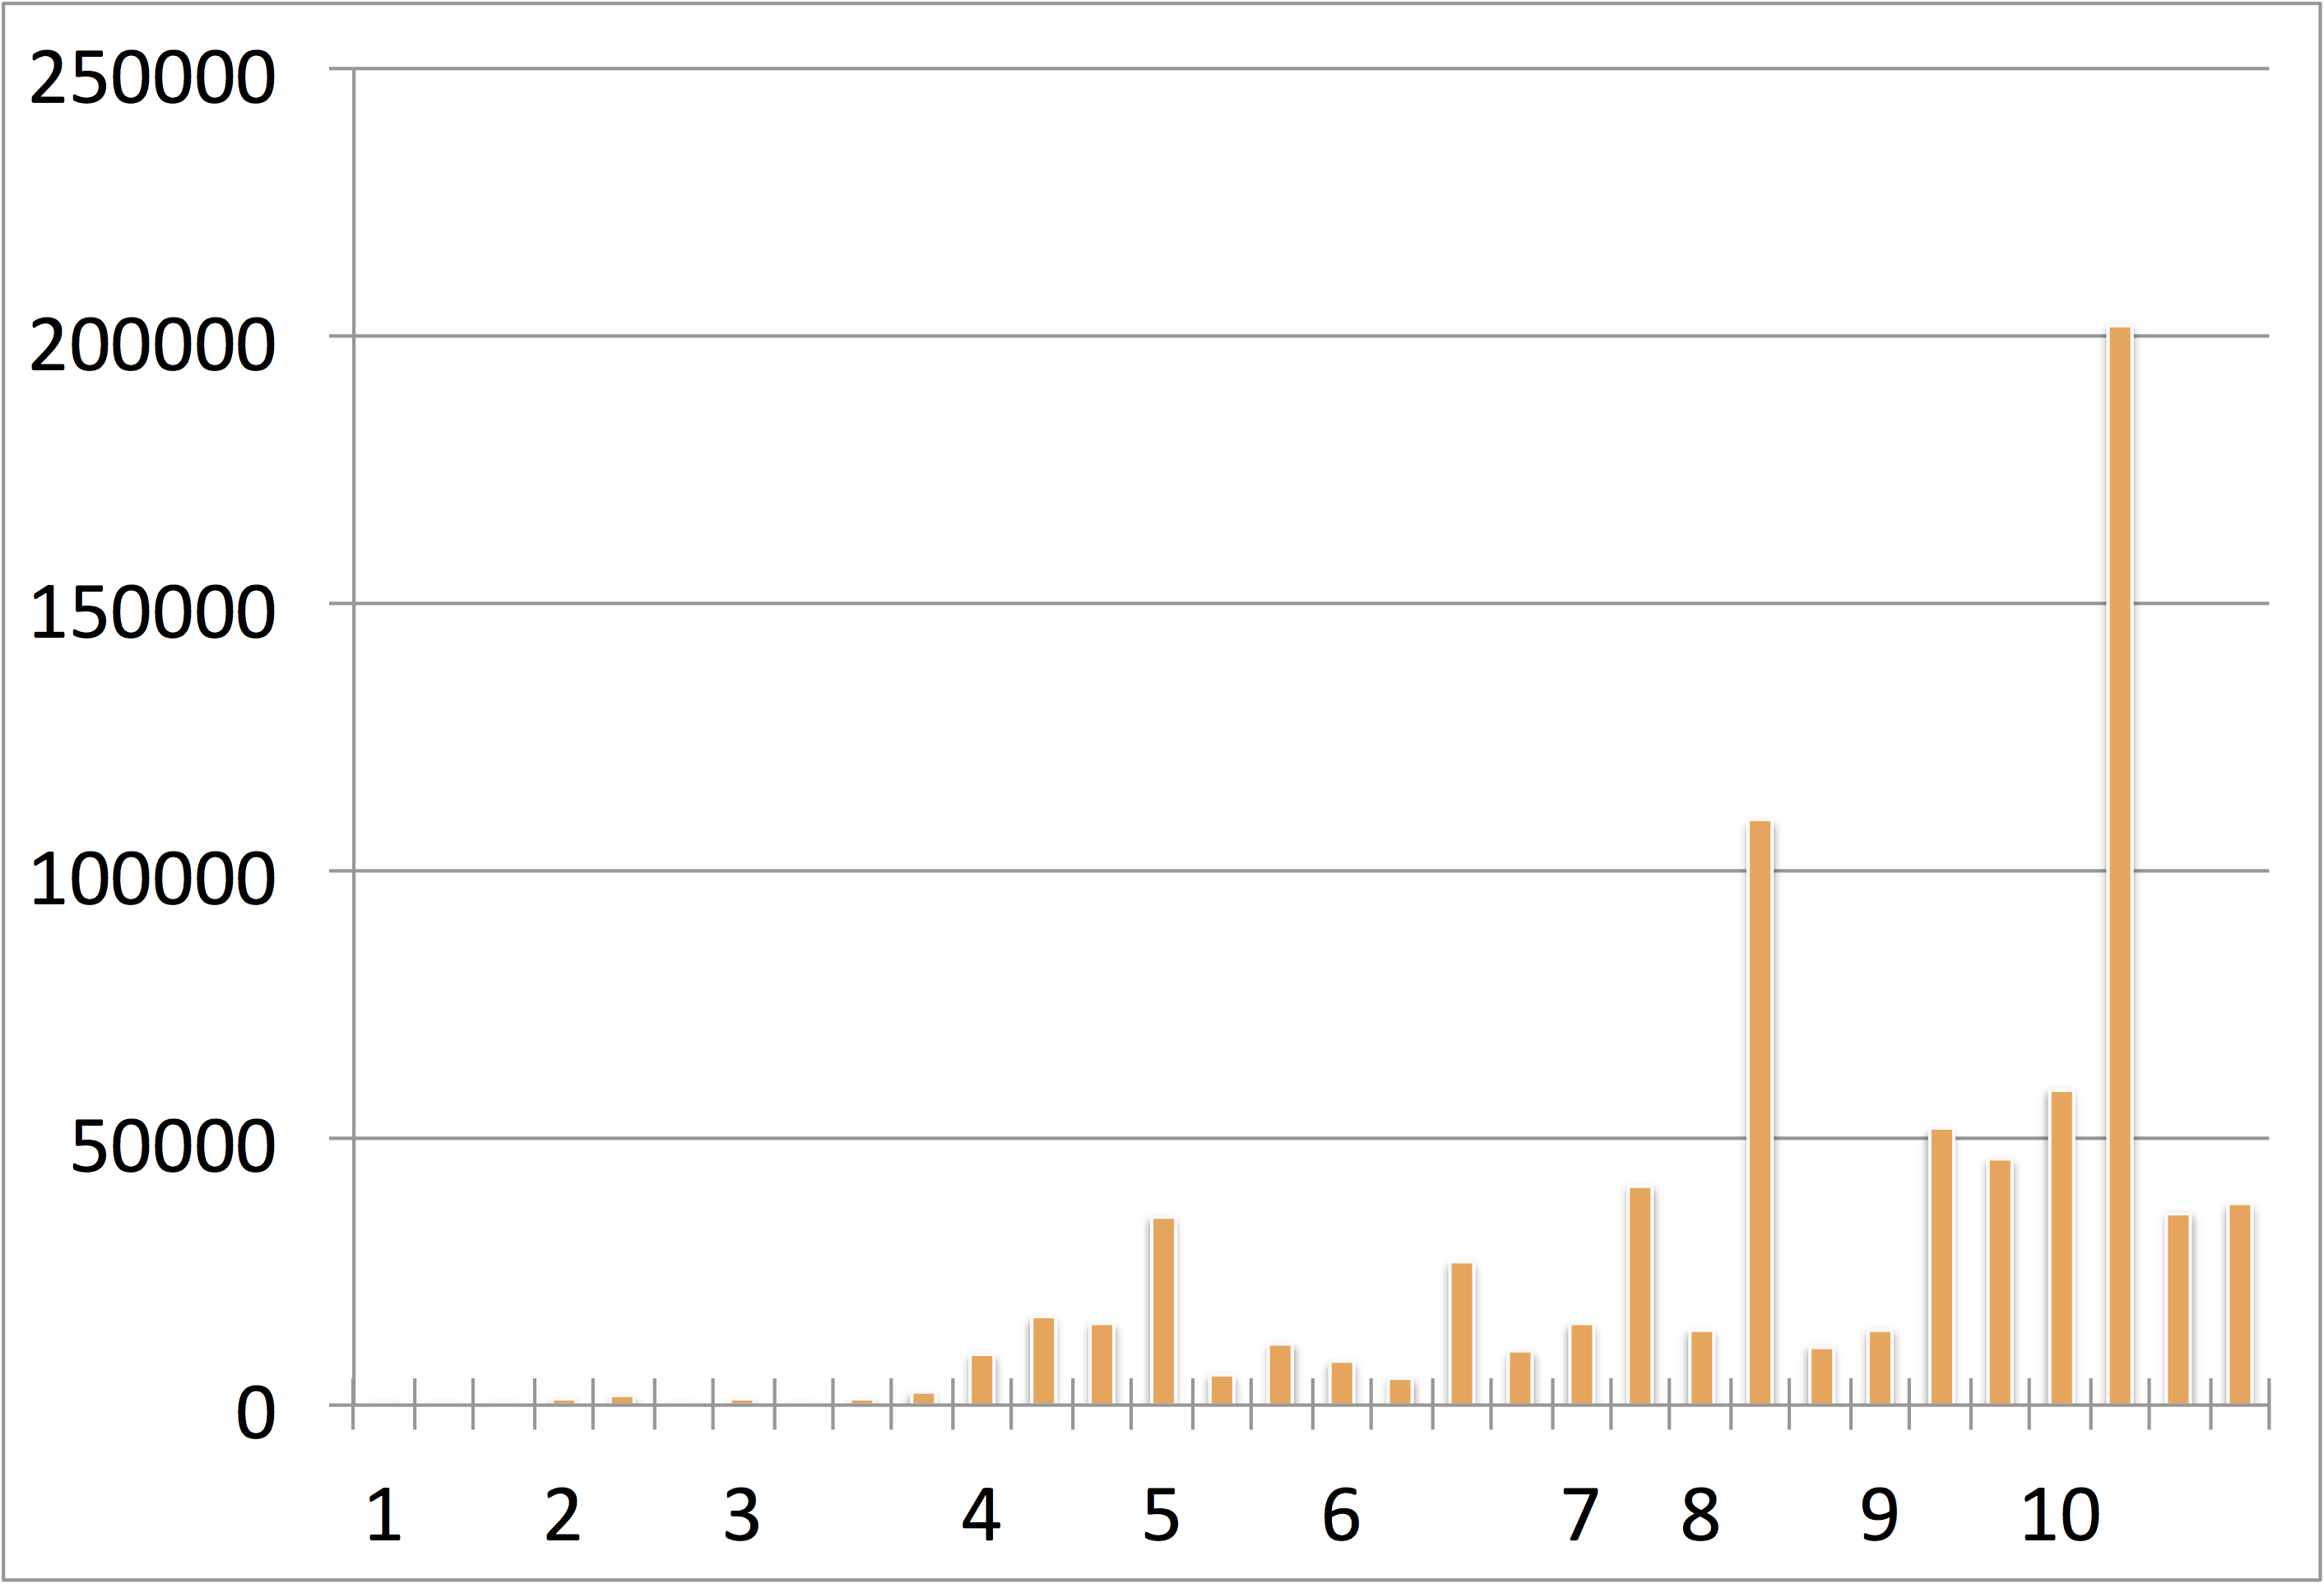
\includegraphics[width=0.8\textwidth]{GradesVsComplexityScores.png}
		\label{image:gradecomplexity}
\end{figure}

\begin{figure}
	\centering
		\caption{The average complexity score of pieces by grade from Royal Conservatory along with standard deviations.}
		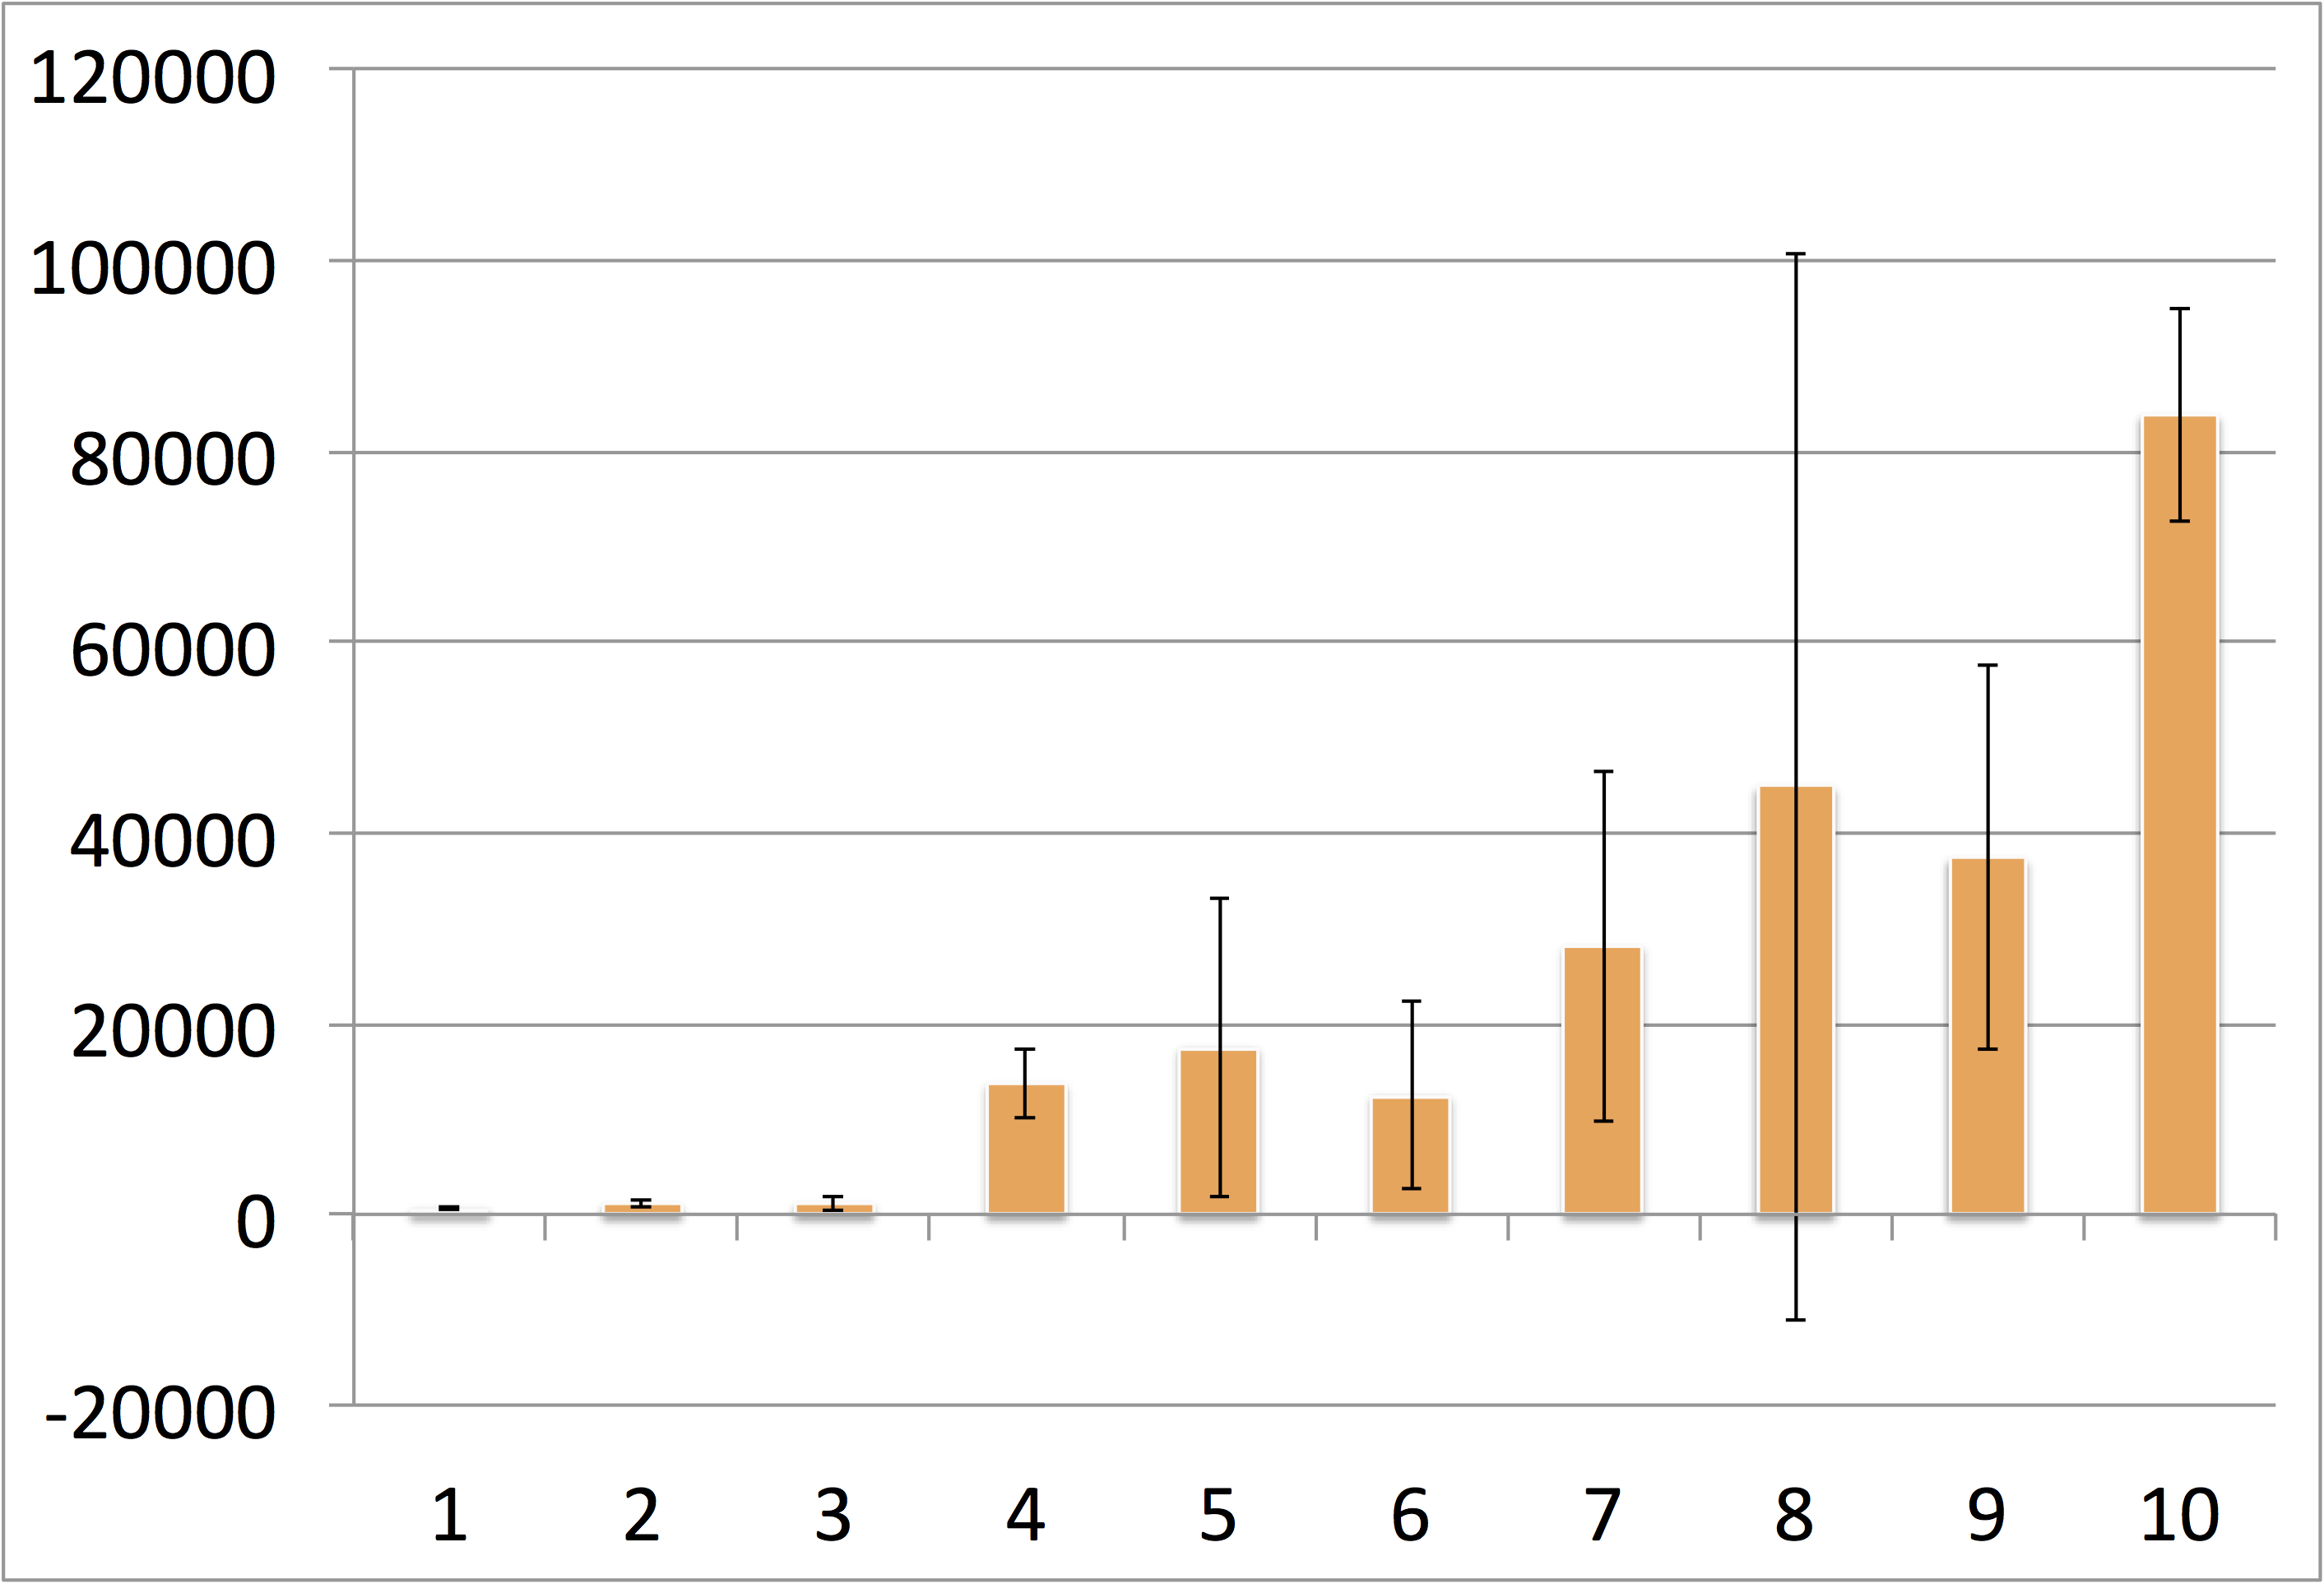
\includegraphics[width=0.8\textwidth]{GradesVsAverageComplexityScoresSTD.png}
		\label{image:gradeaverage}
\end{figure}

\section{Optical Character Recognition (OCR)}
\label{sec:ocr}

The ability to use music scores in PDF format would greatly enhance the usability of our reference implementation. However, this ability hinges on the accuracy of the music OCR software that can translate PDF into MusicXML. Hence, I empirically evaluated the accuracy of a widely used music OCR application to assess its suitability for this system. 

In the experiments, I used freely available music OCR software from Audiveris \cite{Audiveris}. I evaluated the reliability of this process as follows: find pre-matched PDF files with the correct MusicXML, convert the PDF files into a new MusicXML, and finally compare the correct and converted MusicXML to each other.

The pre-matched PDF and MusicXML files used are all from MuseScore \cite{MuseScore} and are listed in Table \ref{table:matched}. They were selected randomly from the list of single part pieces for clarinet. The MusicXML files came in .mxl (compressed MusicXML) format from MuseScore, and they were uniformly imported into Finale Notepad 2012 \cite{FinaleNotepad} to then export the uncompressed format for comparison. For this test I use only Audiveris for conversion.
 
\begin{table}[ht!]
	\centering
	\caption{The works with matched PDF and MusicXML files from MuseScore chosen for testing OCR reliability along with their composer or arranger.}
    \begin{tabular}{| l | l |}
        \hline
    Title & Comp./Arr. \\ \hline
    Dancing Clarinet & KRM \\ \hline
	Mi Razon De Ser & Banda Central \\ \hline
	Rudy & Jerry Goldsmith \\ \hline
	The Hobbit: The Desolation of Smaug & Howard Shore \\ \hline
	The Rose & Dan White \\
        \hline
    \end{tabular}
	\label{table:matched}
\end{table} 

         % Set your language (you can change the language for each code-block optionally)

\begin{figure}[ht!]
	\centering
    \caption{The comparison command for MusicXML files.}
	\lstset{language=bash} 
    \begin{lstlisting}
    sdiff -B -b -s Original.xml OCR.xml | wc
    \end{lstlisting}
    \label{image:sdiff}
\end{figure}

I make use of a file differencing tool with counts of words, lines, and characters as shown in Figure \ref{image:sdiff}, as well as a comparison of complexity scores to highlight the potential effects of the OCR process. I show the difference measurements for select pieces in Figure \ref{image:difference}. I also present the average across pieces for each difference in the same figure. Figure \ref{image:percentage} shows the difference expressed as the percentage of change from the values of the original MusicXML file. It also presents the average across pieces in the same figure.

% \begin{table}[ht!]
% 	\centering
%     \begin{tabular}{| l | l | l | l | l |}
%         \hline
%         Type & Words & Lines & Char's & Score \\ \hline
%         Original & 20964 & 27451 & 580569 & 215546 \\ \hline
%         Converted & 21584 & 30825 & 783894 & 298655 \\ \hline
%         Difference & 10202 & 38200 & 736456 & 83109 \\ \hline
%         Normalized & 0.4866 & 1.3916 & 1.2685 & 0.3856 \\
%         \hline
%     \end{tabular}
% 	\caption{The words, lines, and characters of the original MusicXML, the OCR converted MusicXML, the difference between them, and the normalized difference based on the original.}
% 	\label{table:difference}
% \end{table} 

\begin{figure}
	\centering
		\caption{The difference between matched and OCR generated MusicXML files in words, lines, and characters via sdiff as well as the positive difference in complexity score.}
		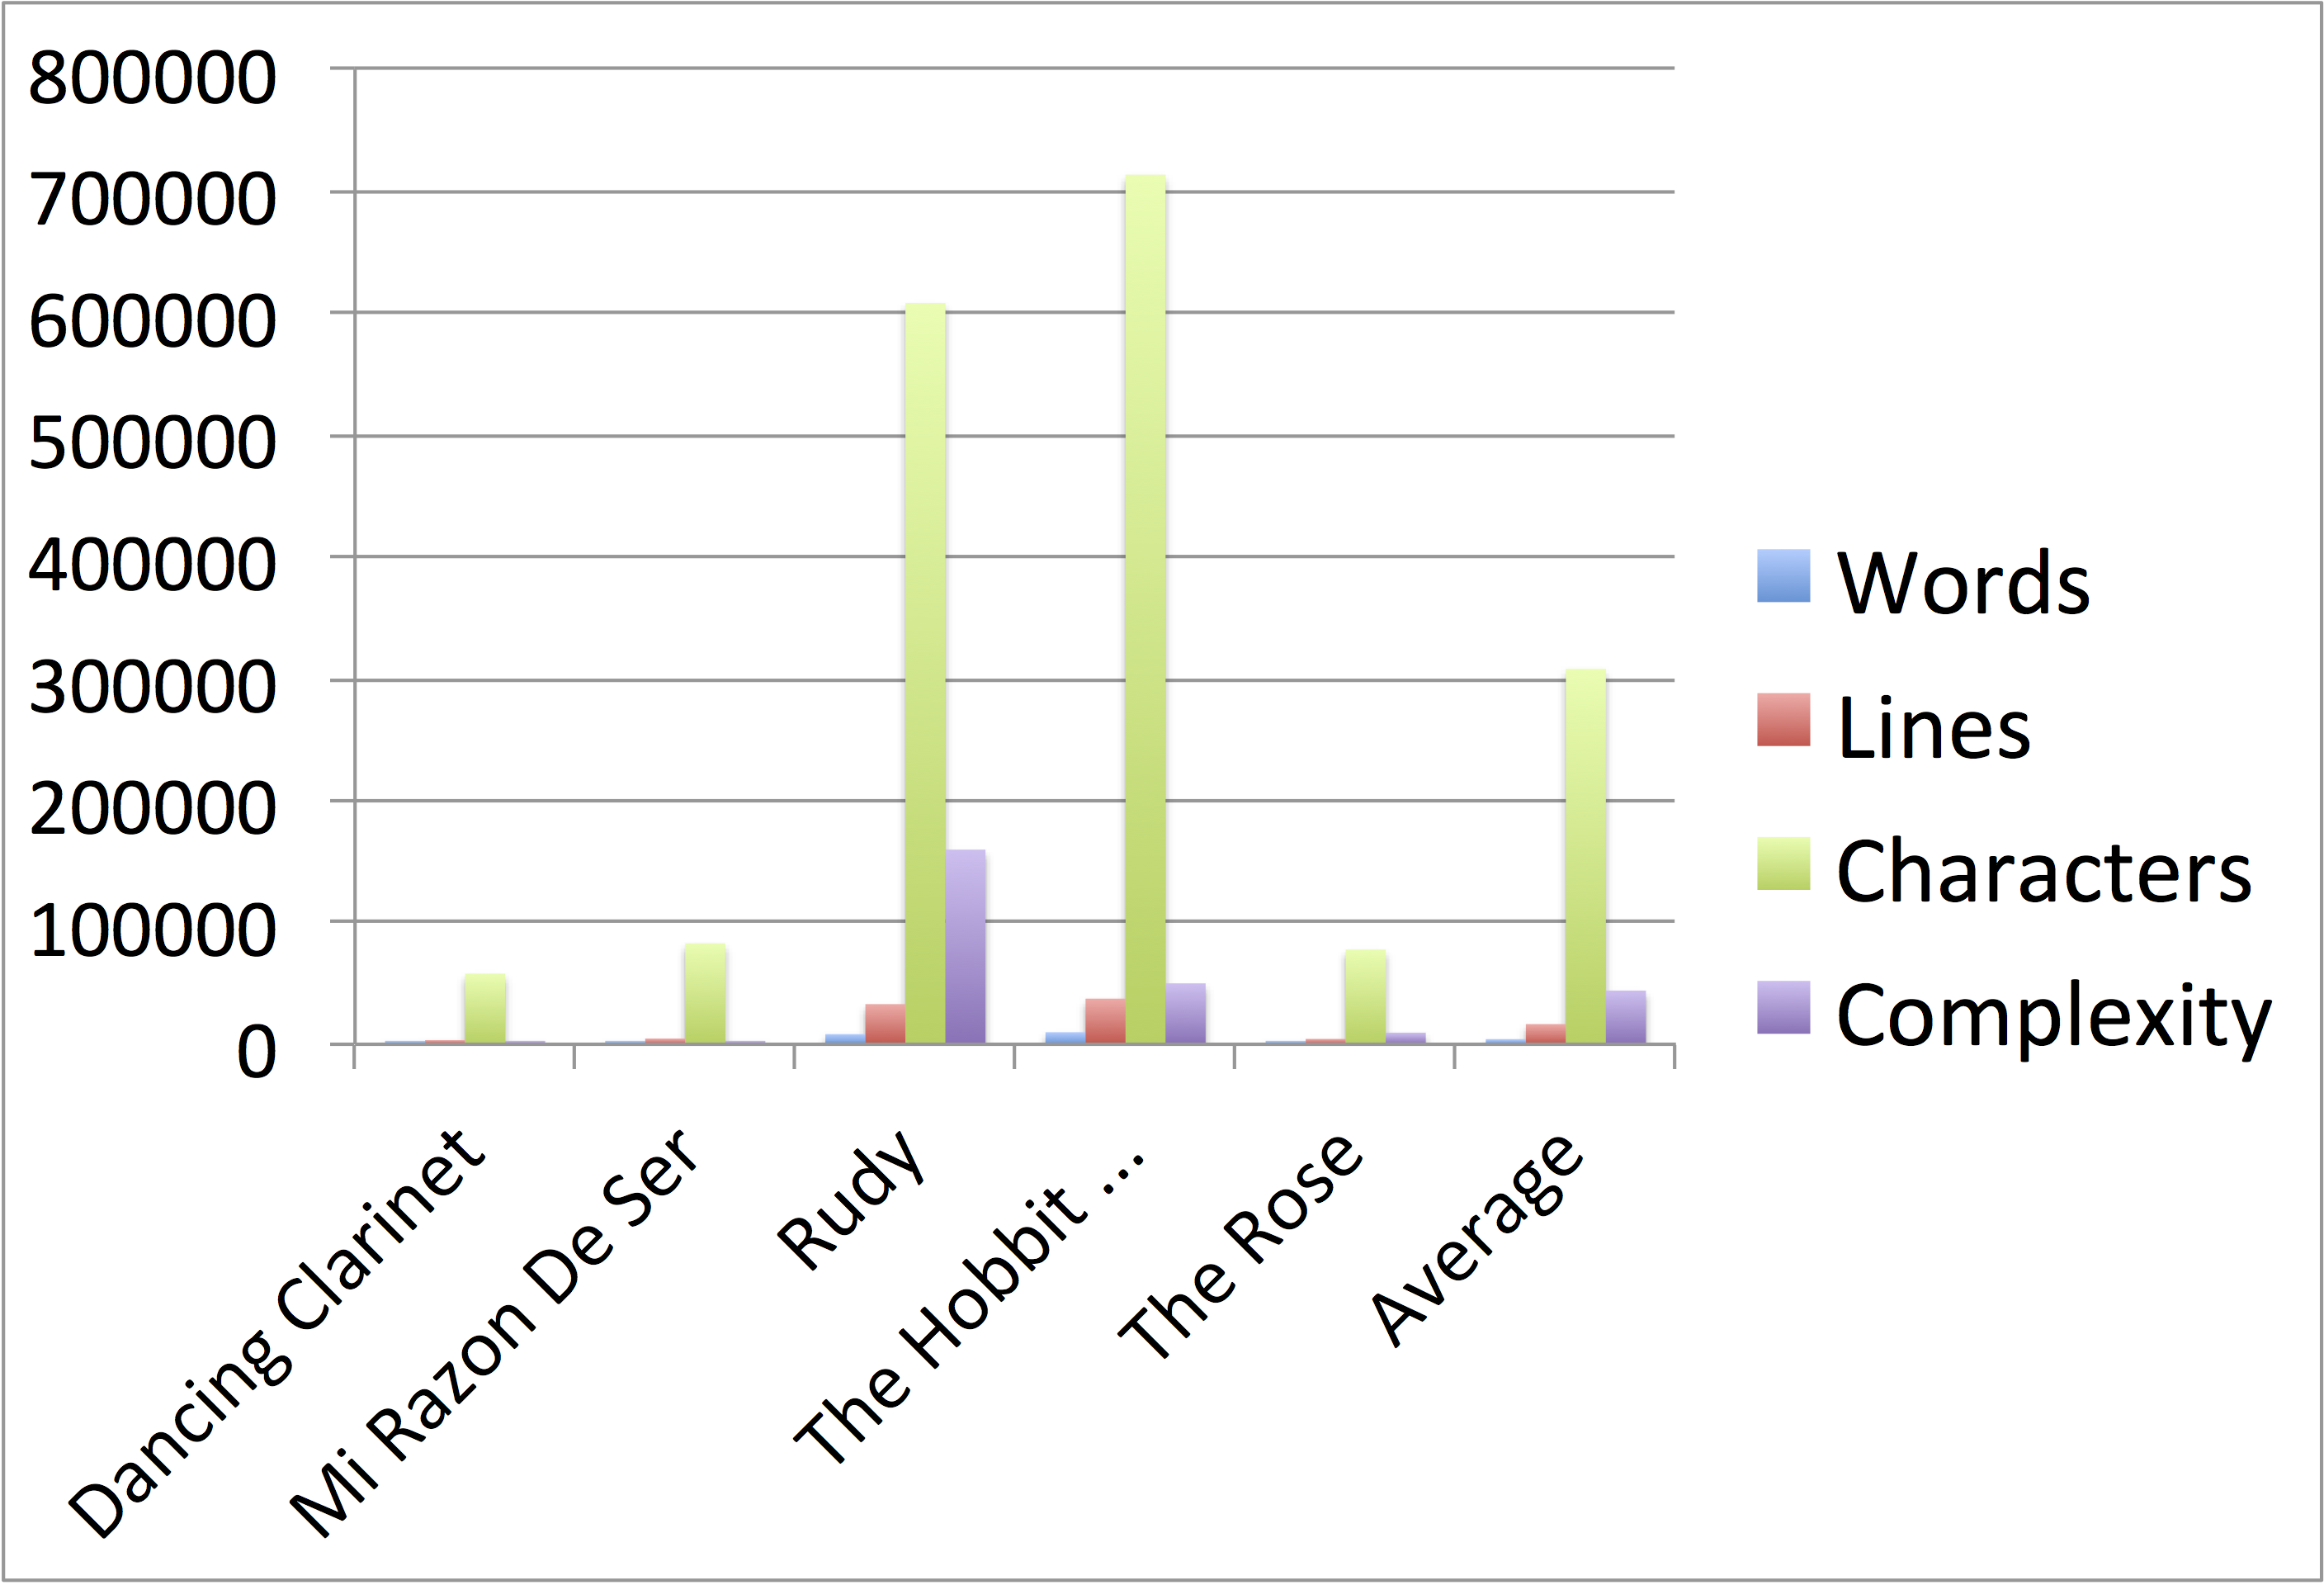
\includegraphics[width=0.8\textwidth]{DifferenceOCR.png}
		\label{image:difference}
\end{figure}

\begin{figure}
	\centering
		\caption{The percentage difference between matched and OCR generated MusicXML files in words, lines, and characters via sdiff as well as the positive percentage difference in complexity score.}
		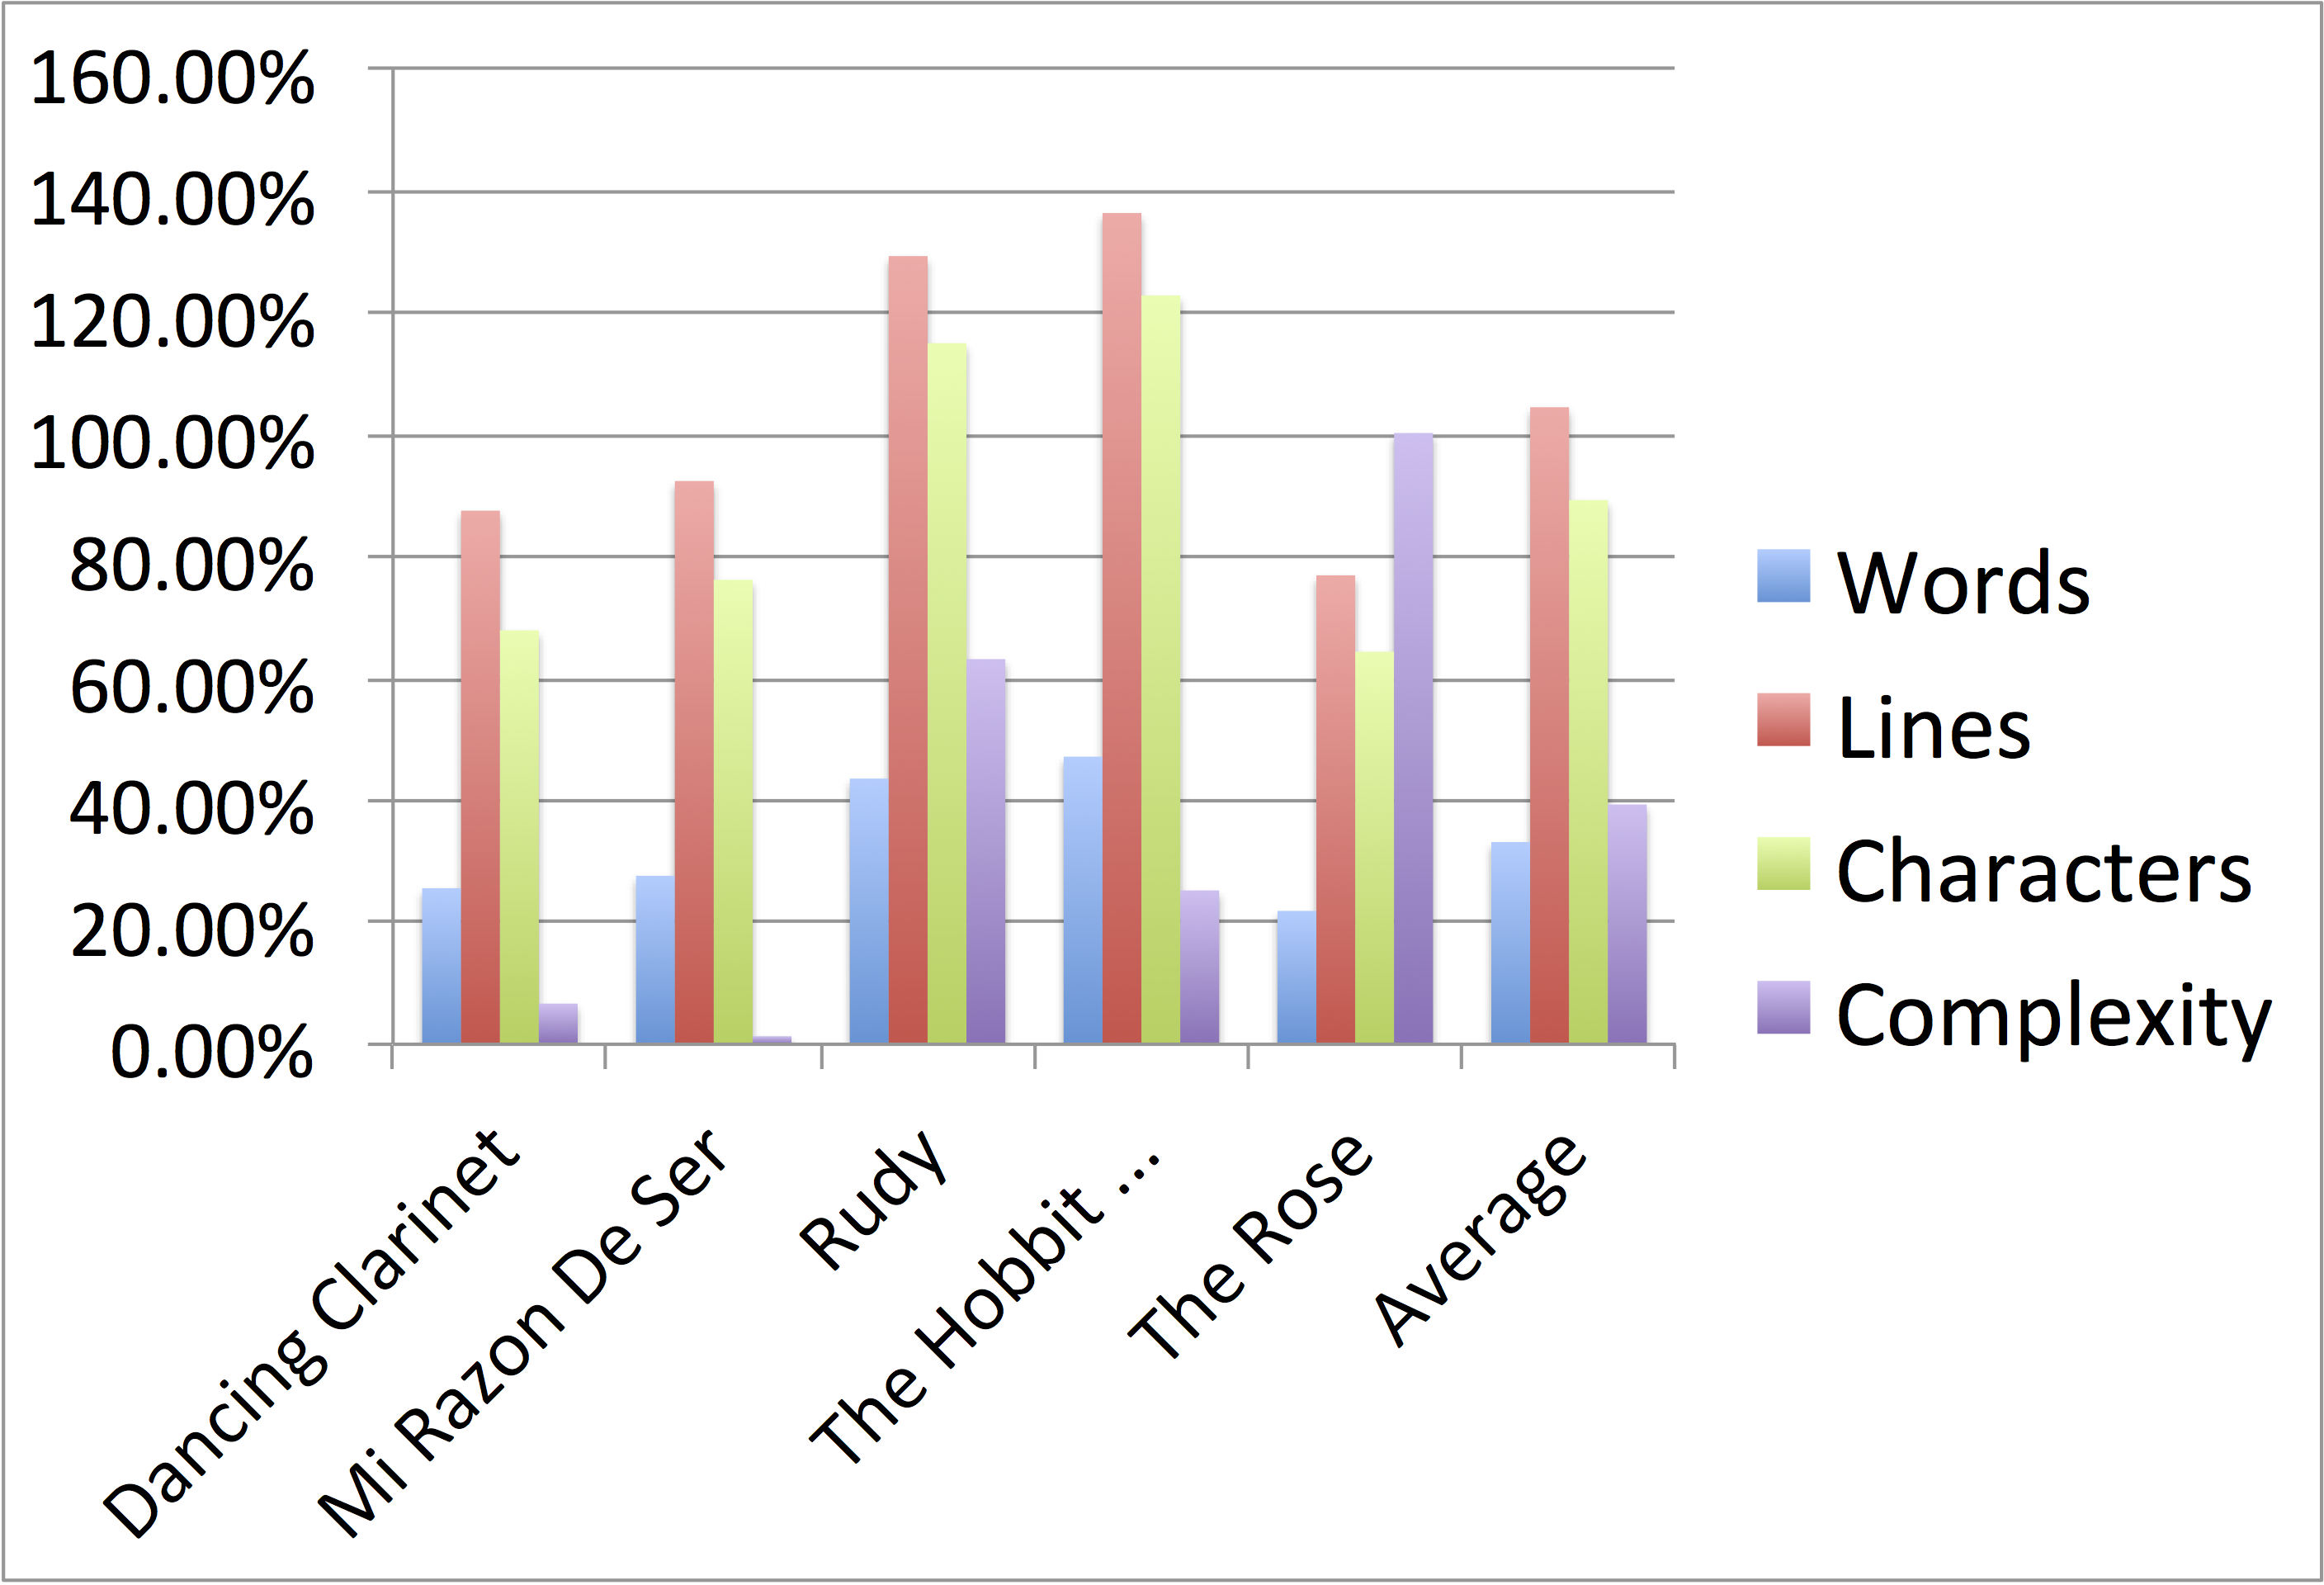
\includegraphics[width=0.8\textwidth]{PercentageOCR.png}
		\label{image:percentage}
\end{figure}

\chapter{Discussion} 
\label{sec:discus}
\markright{Ethan G. Holder  \hfill Chapter 7. Discussion \hfill}

I discuss my findings as follows: Section \ref{sec:grades} covers the results from assessing previously graded pieces from Royal Conservatory; Section \ref{sec:disocr} talks about the results from comparing matched and OCR generated MusicXML files; and Section \ref{sec:usability} discusses the findings with regards to the website's usability.

\section{Manually Graded Pieces and Their Calculated Complexity Scores}
\label{sec:grades}

Figures \ref{image:gradecomplexity} presents the results of applying the reference implementation on 32 scores, which have been manually ranked by music educators as belonging to levels between 1 and 10. 
One would naturally expect the lowest and highest complexity scores to come from grade 1 and grade 10 pieces, respectively. Although the lowest score piece was a higher grade than expected, the second lowest score was indeed for a grade 1 piece, ``Bingo'', and the highest score was for a grade 10 piece, ``Concerto no. 3,'' 2nd and 3rd Movements by Crussell. This outcome shows in one respect, that my results generally correlate with the expectation. Other discrepancies and outliers are to be expected given the subjective nature of grading pieces.


The graph reveals that even though the automatically calculated complexity scores follow the overall trend set by their manual rankings, there is a lot of noise in the calculated scores. This noise reflects the discrepancies between the manual (baseline) and automated (evaluated) rankings. Some outliers are worth examining in detail. In particular, the lowest computed complexity score of 514.19 was for ``Variations on a Theme'' by Mozart, a grade 3 piece, while the highest one of 202214.85 was for ``Concerto no. 3,'' 2nd and 3rd Movements by Crussell, a grade 10 piece. Musicians would argue that music by Mozart is known to be deceptively simple. Hence, the low mechanical difficulty calculated by our tool may not truly represent how human experts see this piece by Mozart, which is a well-understood exception in classical music. The Concerto looks deceptively hard due to the presence of a free-form cadenza that uses the very unusual 17/4 time signature and numerous consecutive tuplets, including both common 16th and 32nd note groups as well as unusual 6-tuplets. It is possible that performers would find this piece much less daunting once they make sense of these rhythms. 


To further illustrate correlation with the expectation, Figure \ref{image:gradeaverage} shows the average complexity score of pieces by grade along with the standard deviation. Here, the complexity scores seem to more closely match what one would expect. The average complexity scores roughly increase and are within one standard deviation of consistently increasing. There are still outliers present, including grade 6 pieces having an average complexity less than grade 5 or 4 pieces, and grade 8 pieces having larger average complexity than those of grade 9. However, all of this evidence is simply a testament to the highly subjective nature of complexity assessment. It is likely that experts presented with the automated results would consider revising their ranking recommendations.

\section{Matched and OCR Generated MusicXML}
\label{sec:disocr}

Another possible explanation for the discrepancies highlighted between graded pieces could be the inaccuracies of the toolchain, specifically music OCR. During the tests, I largely utilized Audiveris \cite{Audiveris} for its simplicity and speed in generating MusicXML as well as its plethora of options for input image formats. However, some files were simply too poor of image quality for it to initially accept. With some manual effort to change image formats and attempts to improve the resolution of scanned images, Audiveris was finally able to catch the remainder of cases.

The process of converting PDF's to MusicXML is admittedly an imperfect means of generating accurate MusicXML representations. As Figure \ref{image:difference} shows, there were large differences between the test bed of matched and OCR generated MusicXML files. The difference in characters is the most alarming, however that could be explained by the limited features OCR is able to analyze with respect to the entire set encoded into the matched MusicXML. Nevertheless, the end result of the file differences leads to the associated differences in complexity scores.

Figure \ref{image:percentage} underscores this difference by showing it as a percentage of the original measure of words, lines, characters, and complexity. While the piece ``Dancing Clarinet'' has only a 6.68\% difference from the original complexity score, the piece ``The Rose'' has over 100\% difference from the original complexity score. Both of these show over 20\% difference in words and over 60\% difference in lines and characters. Interestingly, the pieces ``Rudy'' and ``The Hobbit: The Desolation of Smaug'' both show over 110\% difference in lines and characters, yet the change in underlying MusicXML only causes about 63\% and 25\% difference in complexity for these pieces, respectively.

Therefore, it would seem that the process of using OCR to generate MusicXML from PDF files of music scores is simply not yet mature enough to handle the demands of complex music scores. This conclusion is strengthened by both outside research \cite{byrd2006prospects} and my experience with acquiring such software. The original intention was to deploy such OCR software at the beginning of the control flow from a web UI to allow users to easily upload PDF files without performing a manual conversion on their own. However, of the 5 different OCR packages I experimented with and nearly purchased, most did not even offer an option for batch execution. Those that did offer this option could not operate in this mode consistently or with a measure of reliability.

While this process is obviously imperfect, its speed and automation allow us much more flexibility in generating MusicXML even outside of batch mode. This process is still absolutely necessary for comparing complexity scores of well-known works, since so many have not previously been rewritten into MusicXML. At this point there is no clear substitute for music OCR, but it is my hope that future efforts will strive to improve both the accuracy and reliability of this process so more research can be performed with sheet music.

\section{Website Usability} 
\label{sec:usability}

I do not provide any empirical data so far on the performance of the deployed implementation, but it is publicly available for general use. In informal discussions with potential users, I uncovered many points of design that I discuss here.

First, the website must provide access to the matched PDF file as well as the complexity score from the MusicXML representation. The PDF file is made available so that there is no confusion about exactly what the piece of music is that is generating the score.

Second, I found that many users especially wanted to see what the most complex measure is in the piece as a means of determining whether the complexity score was due to one very difficult spot or a collection of many less difficult areas. Thus, I determine the complexity score for each individual measure in the pieces available. I not only show the measure number and associated score however, I also utilize VexFlow \cite{VexFlow} to graphically represent this measure to further accommodate users.

Finally, the website also features the ability to run on music pieces with multiple parts or instruments. The relevant data for each part or instrument is extracted and even graphed against one another through D3 \cite{D3}. This comparison is not necessarily correct, given that each part or instrument is assigned a complexity score based off of parameters for B$\flat$ Clarinet. Yet, it is still a valuable design point to show the general applicability of this approach to works that are not only for instruments besides B$\flat$ Clarinet, but also for entire ensemble or orchestral pieces.

\begin{figure}
	\centering
		\caption{The main page for the website with user controls.}
		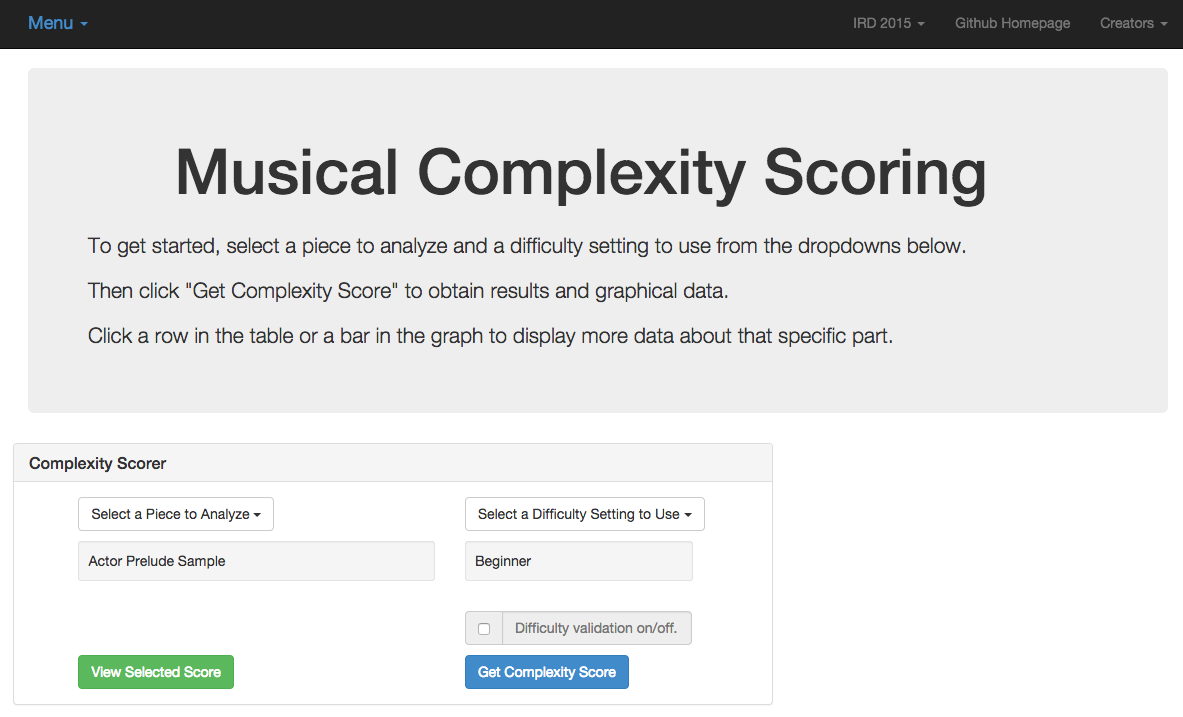
\includegraphics[width=0.9\textwidth]{WebsiteLandingInput.png}
		\label{image:websitemain}
\end{figure}

\begin{figure}
	\centering
		\caption{The table output of complexity data on the website.}
		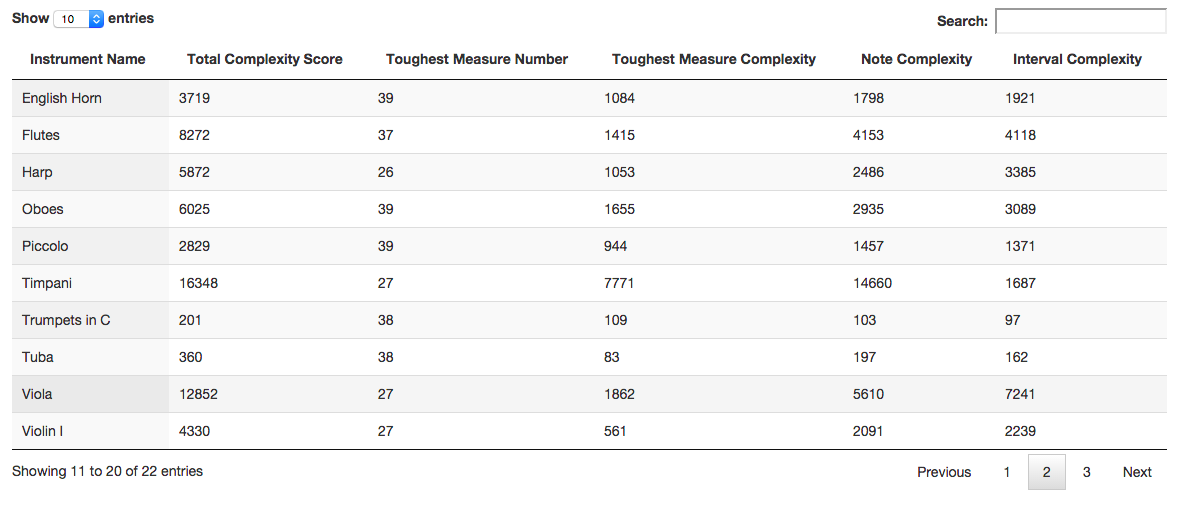
\includegraphics[width=0.9\textwidth]{WebsiteTable.png}
		\label{image:websitetable}
\end{figure}

\begin{figure}
	\centering
		\caption{The graph output of complexity data on the website.}
		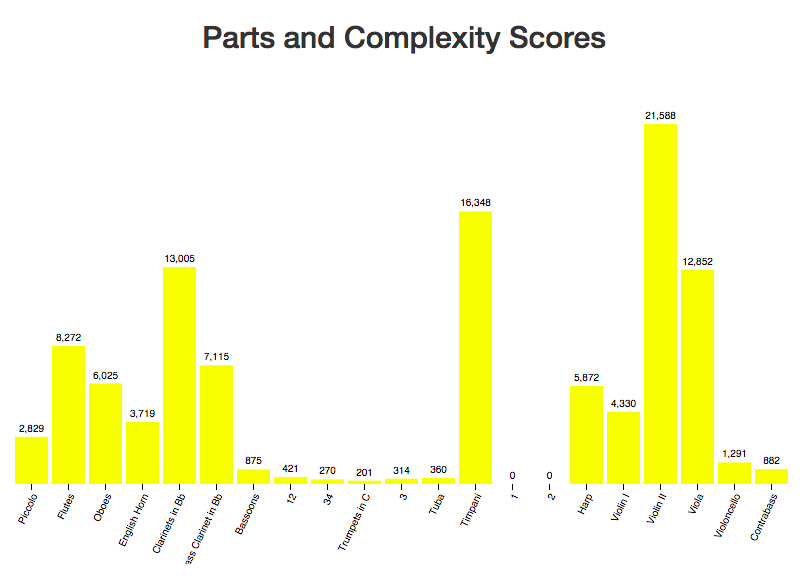
\includegraphics[width=0.9\textwidth]{WebsiteGraph.png}
		\label{image:websitegraph}
\end{figure}

\begin{figure}
	\centering
		\caption{The detailed output for one part on the website.}
		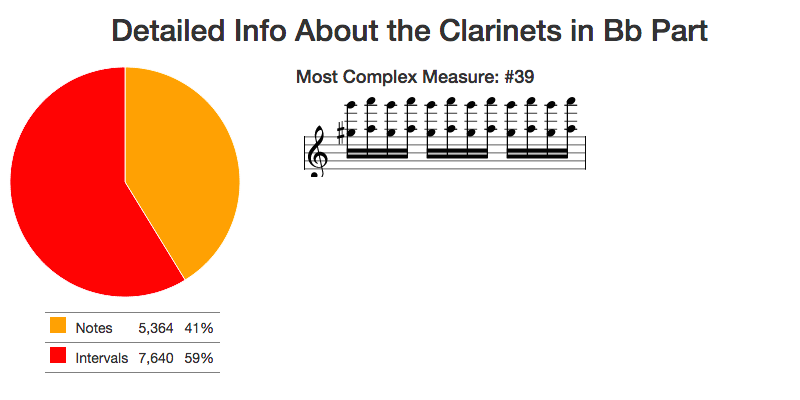
\includegraphics[width=0.9\textwidth]{WebsiteDetails.png}
		\label{image:websitedetails}
\end{figure}

\chapter{Future Work} 
\label{sec:future}
\markright{Ethan G. Holder  \hfill Chapter 8. Future Work \hfill}

The following Subsections address planned future work in a number of different directions, including expanding complexity parameters in \ref{sec:parameters}, mapping parts and instruments in \ref{sec:partinstruments}, understanding complexity scores in \ref{sec:understand}, integrating scores with sources in \ref{sec:integration}, demonstrating this work in \ref{sec:icat},
including more input formats in \ref{sec:input}, measuring complexity from physiology in \ref{sec:physio}, and broadening the approach in \ref{sec:broad}.

%Outline plans to survey more people and expand difficulties for parts.

%Also talk about the point Jason raised in the reading group: reverse engineer this setup and use some creative linear algebra to determine what parameters would be necessary in order for the rankings of state repertoire pieces to match up correctly. As in, given some 1-5 rankings, determine what difficulty settings we need for this method to output complexity scores that fit within 1-5 multiplied by some $\alpha$ that scales the values up and within some range $\beta$ that gives a plus or minus from the scaled values. Tighten up $\beta$ as much as possible.

\section{Expanding Instrument Complexity Parameters}
\label{sec:parameters}

As mentioned in \ref{sec:survey}, the current complexity parameters lack validation. One way to improve their accuracy is thus to gather a consensus from those with a stake in this complexity measurement, such as experts, performers, and educators. I have already begun the process of surveying these people for their opinions on complexity parameters for B$\flat$ Clarinet. However, a notable direction for future work is to expand this survey and indeed the viability of the overall complexity score out to other instruments.

The reference implementation in its current state can run effectively for any instrument, and any complexity parameters can be utilized. In this way it is currently agnostic to what instruments are being played in the piece. I do not attempt here to generate complexity parameters for other instruments (besides B$\flat$ Clarinet) both for brevity and for accuracy. If the approach of surveying stakeholders is practical and viable, then we must expand to utilize it further. If surveying will not work, then we must find another approach to validate complexity parameters.

The alternative to this arranged validation is to allow users to supply their own parameters each time without any set standard. Although this workaround would seem necessary to get customized complexity scores for a given playing level of multiple instruments, it requires potentially specifying all the parameters for an entire orchestra. It is unclear at this point how necessary this feature is compared to a more streamlined process for using the program.

\section{Mapping Separate Parts and Instruments}
\label{sec:partinstruments}

A related tangential point of future work to gathering more instrument complexity parameters is to separate out different parts and instruments so that each can have its own complexity parameters applied. As mentioned before, the reference implementation does not currently differentiate one part from another. Each part in a musical piece has the complexity parameters applied to it equally (as if each part in the piece was for the same instrument and playing level). It is simple enough to separate out these parts, but the problem becomes matching them to standard complexity parameters.

Within an orchestral or similar piece, the different parts can be named a variety of ways by referencing instruments, players, sections, etc. These can be specific or vague, such as ``1st Chair B$\flat$ Clarinet'' and ``High Brass'', respectively. There is no widely accepted, practical standard for how these are specified.

However, we can still attempt to perform this matching. One trivial approach would be to simply keep track of all possible part names the reference implementation ever encounters and periodically update a table that matches the part name in the piece to a set of complexity parameters. A more elegant approach could be to apply some natural language processing techniques to attempt to automatically match the two or, at worst, provide a small subset of alternatives that a user could choose from when running the tool. Yet another alternative could simply be to allow the user to choose exactly which complexity parameters to use for each part at every run. Each of these has its drawbacks in efficiency, usability, and expressiveness. Nonetheless, this problem looms as we move towards more complexity parameters and remains an open area of research that we plan to address.

\section{Understanding Complexity Scores}
\label{sec:understand}

One potential issue users face is that to understand a complexity score requires referencing other complexity scores. For instance, the score of 1000 for some piece (or part equivalently) X cannot be meaningfully interpreted without knowing what that piece is, such as a Mozart symphony, or knowing other scores of pieces, such as a Beethoven symphony scoring only 500 so piece X is twice as complex.

One possible solution for this problem is to track the names of pieces (and parts) along with their complexity score in a database. Then, upon scoring some piece, the reference implementation can also output the closest scores of well-known pieces, thus providing a reference point. While keeping track of these scores in a database may also help speed up computation by not repeatedly calculating the score for the same piece over and over, this introduces much more overhead if users are allowed to input any complexity parameters.

Another solution to this problem would be to scale the score down to some range of numbers, such as 0 to 100. Scaling would mean that no piece could have a complexity score greater than 100 or less than 0. While this may not directly solve the problem of understanding the complexity score, it does bound the possible scores and thus provide its own reference point.

This approach may be more useful for competition rankings so that the complexity score can be easily factored into the score for a performance. However, there is no simple way to scale all complexity scores down without knowing what would receive the highest possible score. Knowing the potential highest score becomes an even more difficult task with user supplied complexity parameters that can wholly change the resulting complexity scores. We are nevertheless investigating this currently to see how we could at least limit scores to some arbitrarily high value and scale based on that.

\section{Integrating Complexity Scores with Sources}
\label{sec:integration}

To make musiplectics more accessible, one direction for future work lies in integrating the complexity score into various music applications. For instance, we envision notation applications, such as Finale Notepad \cite{FinaleNotepad} or Sibelius \cite{Sibelius}, displaying the complexity score of a piece as it is being written so composers can readily see exactly how complex their piece is numerically. Similarly, we would like to partner with music sharing websites, such as International Music Score Library Project \cite{IMSLP}, that allow users to search, view, and download pieces of music. We envision the complexity score of a piece being available before downloading, or more importantly purchasing, the piece so as to give users some reassurance of what they are getting. This could also lead to users being able to search pieces by their complexity score (if they were pre-computed and stored somewhere) should the user need to find a piece to match his or her playing level.

\section{Demonstrating Musiplectics for Art Expos\'e}
\label{sec:icat}

Virginia Tech's Institute for Creativity, Arts, and Technology (ICAT) annually holds an expos\'e for new research and works of art that combine technology with the arts in a variety of ways. ICAT Day as it is called will serve as a formal demonstration for many potential stakeholders to see Musiplectics in action and get to interact with the reference implementation. In order to facilitate this interaction with the reference implementation, some minor changes were made to the frontend web interface, turning it into a sort of game for spectators to play.

As shown in Figure \ref{image:websitegameinput}, the game format of the web page allows users to input their best guess for what the most difficult measure is within the piece. For pieces with only a single part, this is relatively straightforward. For pieces with multiple parts, the guess is applied uniformly to all parts (users cannot make multiple guesses for each part). The request sent to the backend is identical to before, but once the response is returned, the most difficult measure for each part is compared to the user's guess. If the guess is correct, output such as in Figure \ref{image:websitegameoutput} is shown over top of the results. If the guess is incorrect, similar output is shown with the correct measure for each part.

\begin{figure}[ht!] 
	\centering
		\caption{The modified input for the game version of the website.}
		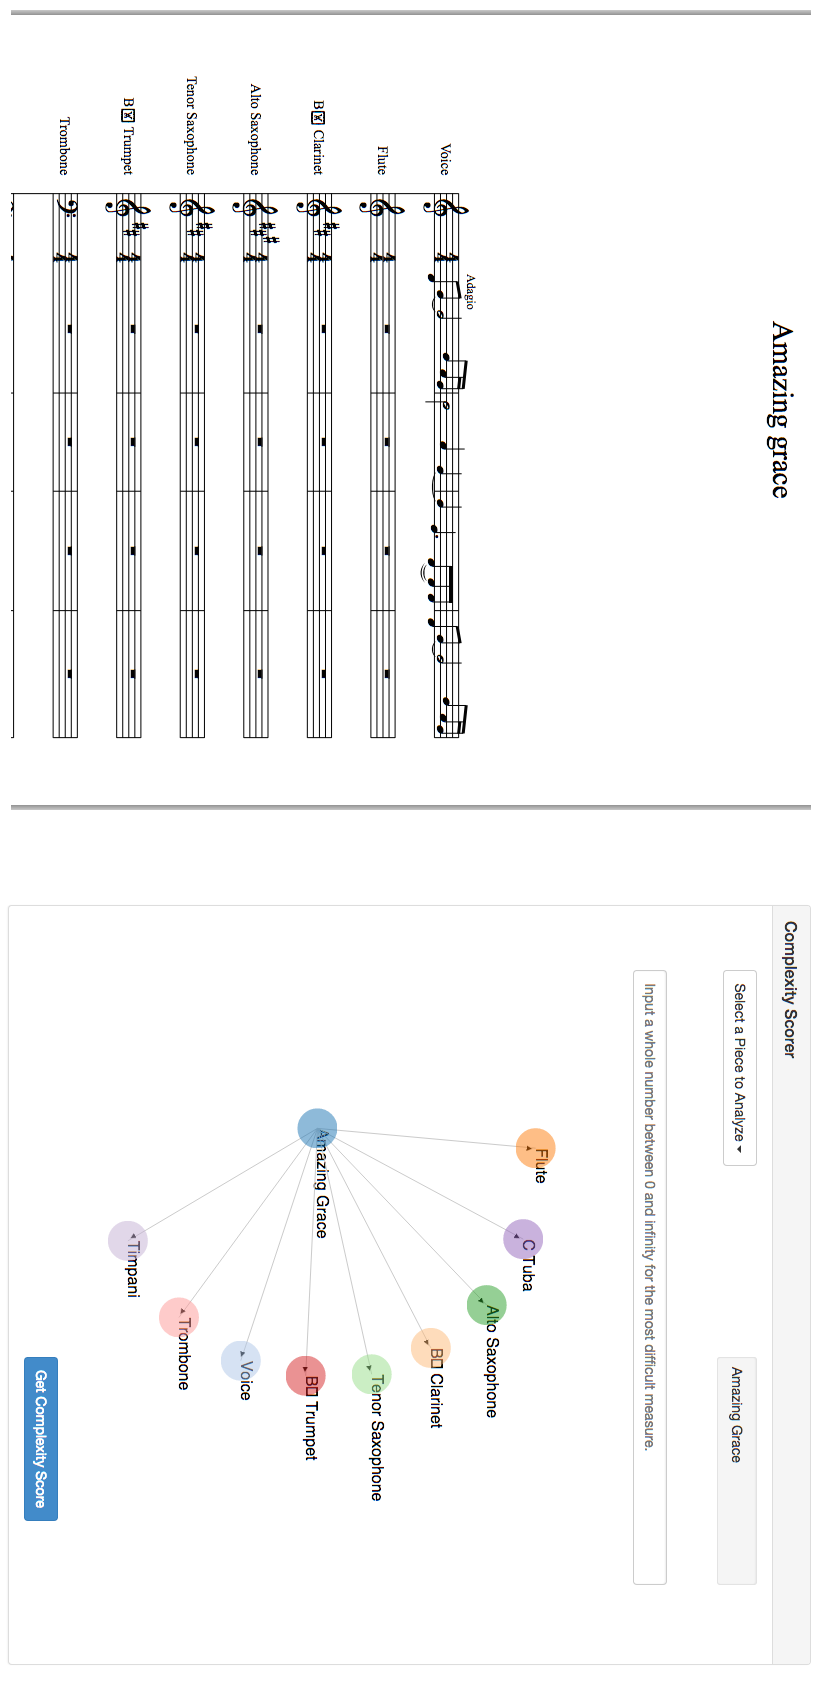
\includegraphics[width=0.9\textwidth]{WebsiteGameInput.png}
		\label{image:websitegameinput}
\end{figure}

\begin{figure}[ht!]
	\centering
		\caption{The potential output for the game version of the website (using Google Chrome \cite{chrome}).}
		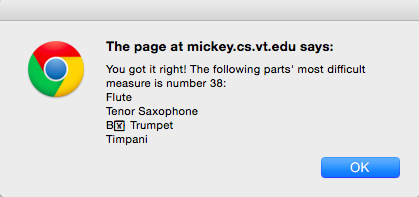
\includegraphics[width=0.9\textwidth]{WebsiteGameOutput.png}
		\label{image:websitegameoutput}
\end{figure}

During ICAT Day, I plan to informally assess the accuracy of the musiplectics approach compared to the expectations of potential stakeholders. While no formal data collection or analysis will be performed, this demonstration should provide critical insights and user suggestions. These can further allow us to improve the usability of the web page and accuracy of the overall approach.

%some stuff goes here \cite{Seemore}

\section{Including More Input Formats}
\label{sec:input}

Yet another direction for future work is the expansion of the formats that can be input in general. At the moment MusicXML files are of course supported, and PDF files can be manually translated to MusicXML via OCR. As mentioned above, this process is not yet mature enough to be run automatically, but OCR in general can operate on many other formats, such as PNG, TIFF, and BMP images, so it would be trivial to expand to allow those inputs.

Beyond what OCR can handle, even more inputs can be translated into MusicXML. Software, such as NotationSoft \cite{NotationSoft}, can translate event-driven MIDI files \cite{midi1996complete} into MusicXML. This type of translation could bring a wealth more of input since a large amount of music literature is stored in this fashion. In fact, efforts such as \cite{Choudhury2000} are already taking place to digitize a large amount of publicly available music into MIDI. An extension to incorporate translated MIDI files would greatly expand the applicability of musiplectics.

\section{Measuring Complexity From Physiological Signals}
\label{sec:physio}

Some prior work has focused on measuring physiological characteristics, especially in the field of human-computer interaction. Often these measurements have been used as indicators of emotional state \cite{Physio}. In relation to music, these measurements have been used both to gauge an audience's reaction to a piece of music \cite{chapados2008cross} \cite{gomez2004affective} as well as a means for people to play their own music \cite{Controller} \cite{Tanaka2002}. We would like to leverage these types of works to incorporate physiological measurements and biofeedback as a means of forming or validating complexity scores.

The knowledge of a performer's relative playing proficiency combined with their basic physiological traits while playing a piece could form a model for extrapolating the cognitive load or mental complexity being endured. This method can become a reliable means of parameterizing our system for individual players.

Additionally, future research could compare the physiological measures of mental complexity being endured to the expected complexity of the piece of music at any given time. It is our belief currently that performers tend to become more anxious (and thus endure higher levels of complexity and stress) directly before a particularly complex part of a song. Thus, we would expect to find a flip-flop pattern where mental complexity can be measured to increase first, and then the complexity score of the piece thus far will increase second, while the measured mental complexity then decreases (assuming the performer plays the selection of music correctly).

\section{Broadening Musiplectics to Other Plectics}
\label{sec:broad}

Past work in deciphering the human genome showed the promise of computers in being able to handle great levels of complexity and yield insightful results \cite{genomePub} \cite{genomePri}. While musiplectics does not require as much computational power as a task like deciphering human genes, we still draw parallels to the overall approach of decomposing something exceedingly complex for human and allowing computers to aggregate the small parts, thus providing valuable insights.

To that end, another potential area for future work in expanding the core approach of musiplectics to other areas of complexity measurement. Any well-defined task can be decompose into its principle parts. In music, this means separating a piece of music into the elements we described previously. As discussed above, in program performance estimation, this means separating source code into the low-level instructions that execute on a given machine. Analogously, certain activities could be defined in a similar fashion, such as cooking. In cooking, this would mean decomposing a dish into the steps and ingrediants required to create the dish as well as assigning values or weights to each step in the process. This process is already performed to some degree to estimate the time required to create a dish, but it could similarly be extended to estimate the overall cost or the difficulty of preparing the dish.

There are many other genres of plectics that could apply this approach. It is not yet clear how formally defined a process must be to effectively make use of this approach, but it is our belief that tasks specified by both natural and formal languages \cite{kamp1993discourse} \cite{harrison1978introduction} \cite{kate2005learning} could benefit from these types of insights.

%Talk about using this for other tasks, both understood (sports) and specified, via natural (work tasks, mechanical turk) or formal (music, enterprise project planning) language.

%Draw inspiration from bioinformatics \cite{genomePub} \cite{genomePri}.

\chapter{Conclusions} 
\label{sec:conclu}
\markright{Ethan G. Holder  \hfill Chapter 9. Conclusions \hfill}

This paper presented musiplectics, a new computational paradigm, that systematically evaluates the relative difficulty of music scores, thus benefiting educators and performers. Our hope is that musiplectics can improve the landscape of assessment of music scores. The work presented here unveils our first steps towards an objective and automatic approach to computing the complexity of music pieces. The contributions of this paper include our model for computing complexity scores and its concrete realization in our reference implementation. The automatically computed complexity scores of many well-known pieces and their respective manual grades demonstrate the promise of musiplectics to alleviate the burden of music complexity rankings, freeing musicians for more creative pursuits. In addition, future work directions present many exciting opportunities to apply computing to solve important problem in music arts.

%%%%%%%%%%%%%%%%%
%
% Include an EPS figure with this command:
%   \epsffile{filename.eps}
%

%%%%%%%%%%%%%%%%
%
% Do tables like this:
%\markright{Ethan G. Holder  \hfill Chapter 4. Computational Model for Music Complexity \hfill}

%  \begin{table}
%  \caption{The Graduate School wants captions above the tables.}
% \begin{center}
%  \begin{tabular}{ccc}
%  x & 1 & 2 \\ \hline
%  1 & 1 & 2 \\
%  2 & 2 & 4 \\ \hline
%  \end{tabular}
% \end{center}
%  \end{table}

%%%%%%%%%%%%%%%%%%%%%%%%%%%%%%%%

% If you are using BibTeX, uncomment the following:

\nocite{*}
\bibliographystyle{abbrvnat}
%\bibliographystyle{abbrv}
\markright{Ethan G. Holder  \hfill Chapter Bibliography \hfill}
%\thebibliography{HolderThesis2015}
\bibliography{HolderThesis2015}

% Otherwise, uncomment the following:
% \chapter*{Bibliography}

% \appendix

% In LaTeX, each appendix is a "chapter"
% \chapter{Program Source}

\appendix

\chapter{Complexity Parameters Example}
\markright{Ethan G. Holder  \hfill Appendix Complexity Parameters Example \hfill}
\label{sec:appcomplexity}

\lstinputlisting[language=xml,caption={The full xml file of complexity parameters for beginner B$\flat$ Clarinet.},label={xmlexample}]{Beginner.xml}

\chapter{External Survey}
\markright{Ethan G. Holder  \hfill Appendix External Survey \hfill}
\label{sec:appsurvey}

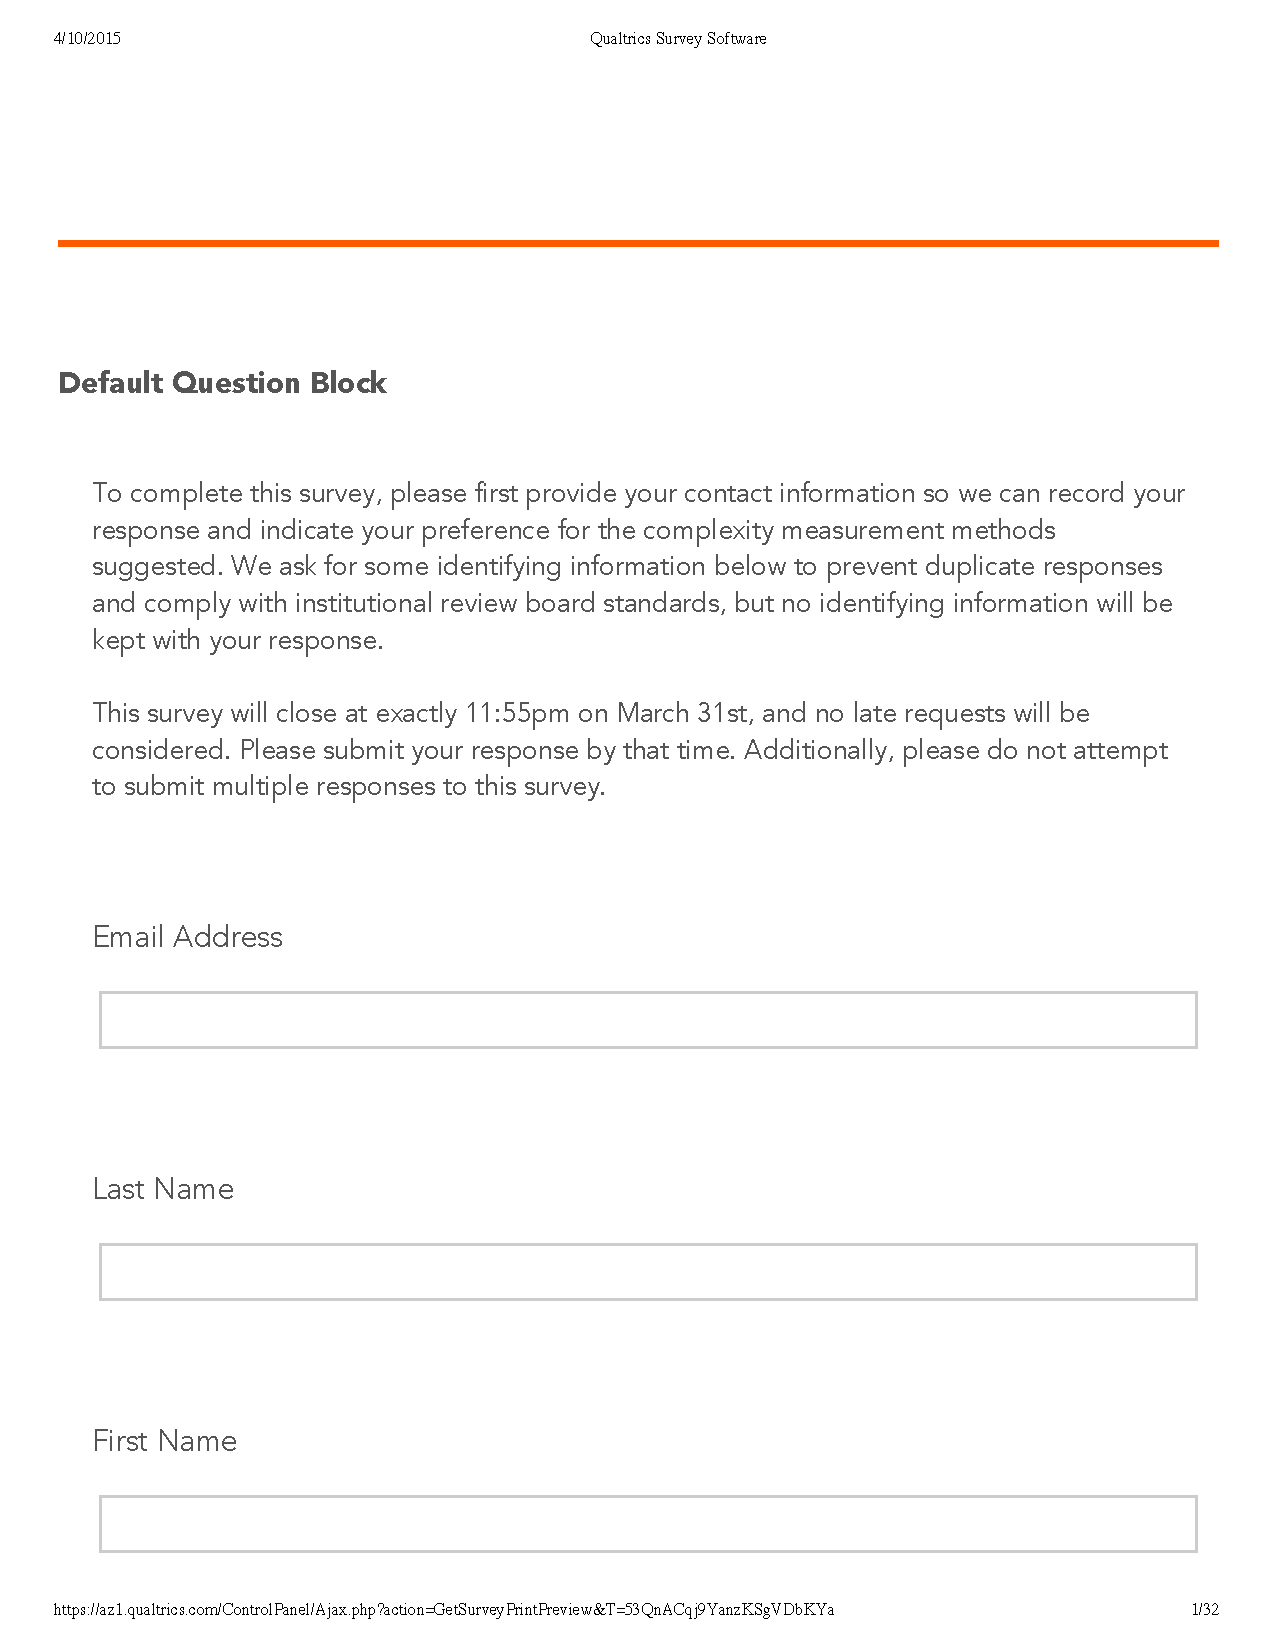
\includepdf[pages=-,scale=.8,pagecommand={}]{MusicScoringSurvey.pdf}
% \begin{figure}[htp] \centering{
% \caption{External Survey}
% 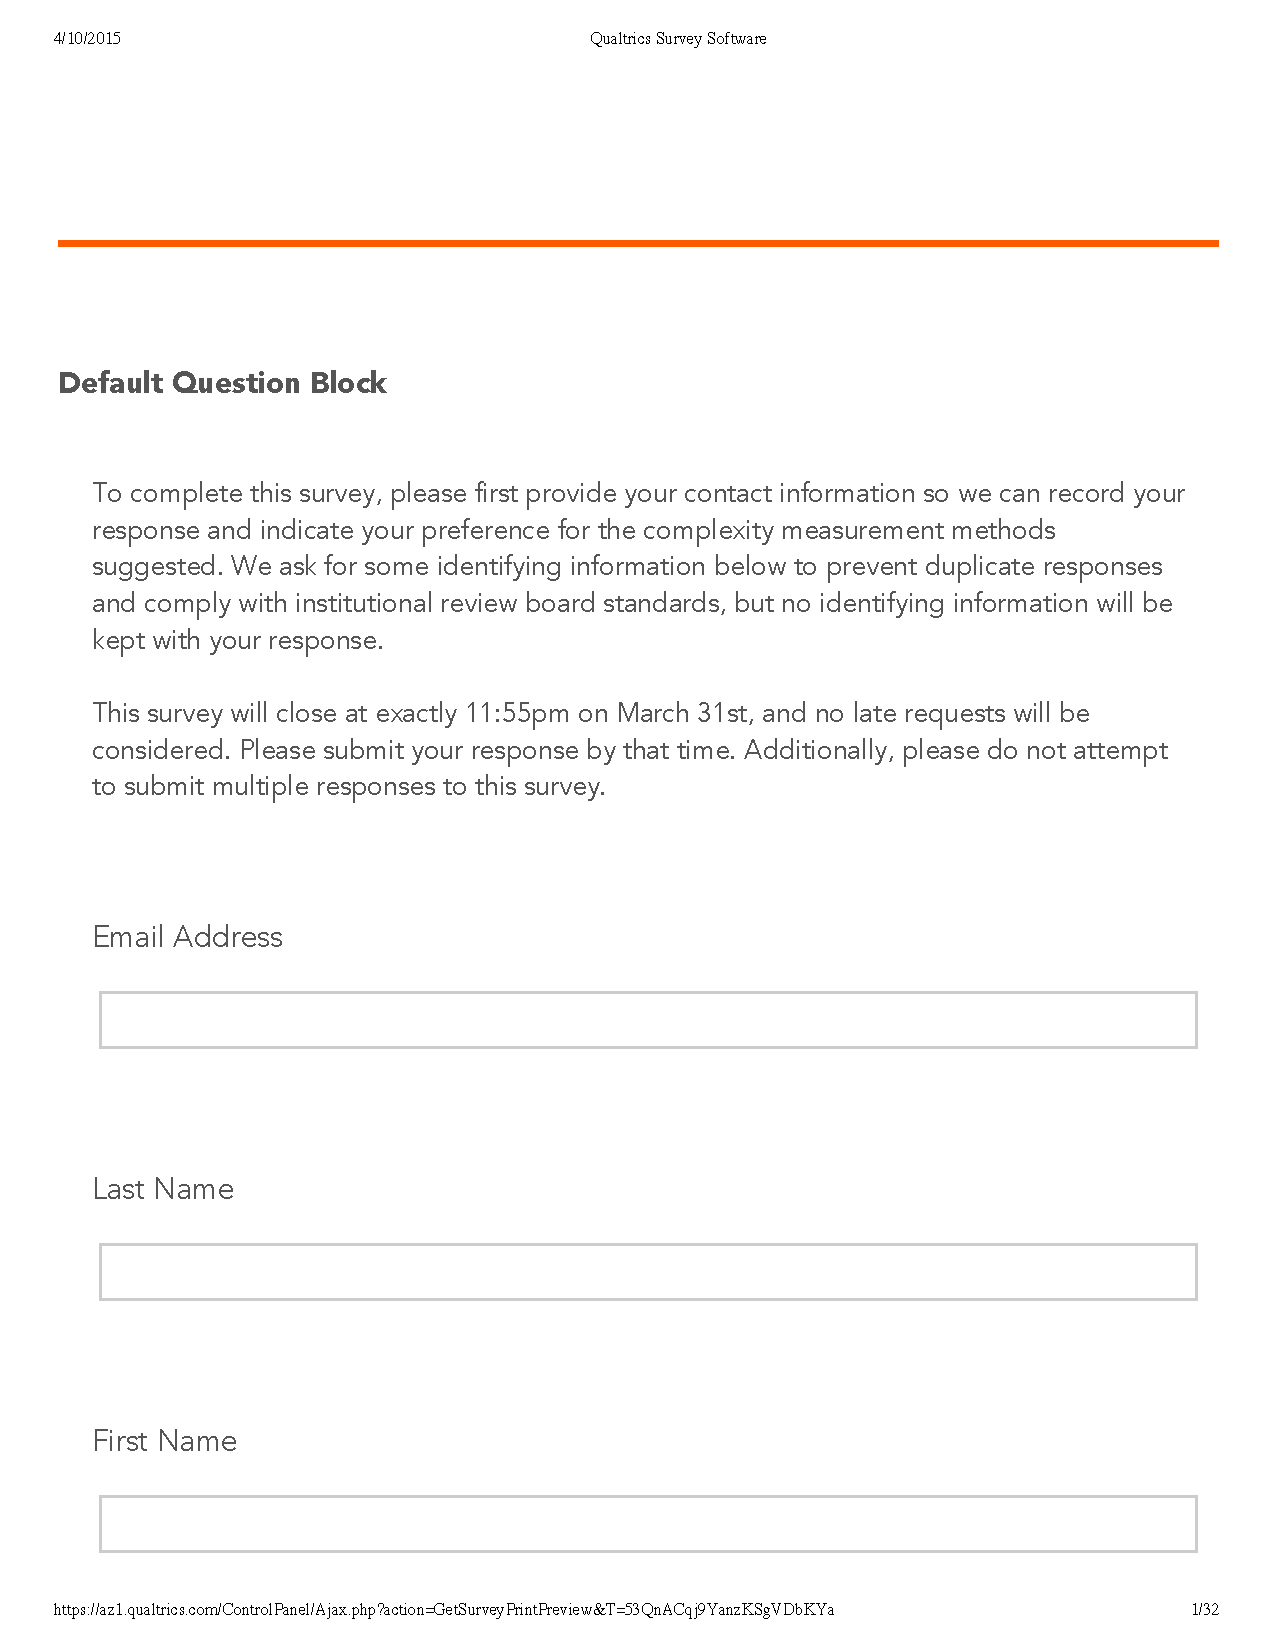
\includegraphics[scale=0.82]{MusicScoringSurvey.pdf}}
% \end{figure}

\end{document}